\graphicspath{{Chapter1/Figs/}}

\section{Introduction}
% ------------------------------------------------------------------------------
%\begin{frame}\frametitle{DSO last year}\framesubtitle{}\label{}
%\vskip-1.5cm
%  Dionysos Satellite Observatory (DSO) of the National Technical University of 
%  Athens (NTUA), has developed and maintains an automated processing
%  scheme to accommodate the routine analysis of all available continuous GNSS 
%  stations in Greece.
%  \\
%  This daily analysis process is implemented for over ten years now (not 
%  always continuous though dues to various problems), yielding 
%  results which help us further understand the complicated tectonic setting of 
%  Greece and nearby regions.
%  \\
%  Updates:
%  \begin{itemize}
%    \item archive old data (from 1995) for reprocessing,
%    \item new network processing (HEPOS) 
%    \item develop PPP-AR PRIDE near real time processing for high rate available data
%    \item start updating for Strain Tool 
%  \end{itemize}
%\end{frame}
%
% ------------------------------------------------------------------------------
\begin{frame}\frametitle{Motivation}\framesubtitle{}
\vskip-1cm
  % Via our contribution to EUREF and interaction with its community, we hope to:
  Routine GNSS processing and site/network monitoring is crucial, because:
  \begin{itemize}
    \item Greece lies in a region of utmost tectonic and volcanic unrest (e.g. 
      active volcano in Santorini isl.),
    \item results \& products are important to a series of fields spanning 
      the whole range of Geosciences,
    \item helps us follow and apply state-of-the-art technologies in GNSS analysis 
      \& Satellite Geodesy and expand \& modernize our research activity,
    \item contribute to the GNSS/EUREF community and be involved in ongoing/future projects,
    \item develop new features for high rate processing.
    \item improve our academic services (NTUA is a University)
  \end{itemize}
  Throughout the last years, routine processing \& monitoring has hepled us gain 
  a more thorough view of the complex tectonic and volcanic setting of Greece.
\end{frame}
%
% % ------------------------------------------------------------------------------
%\begin{frame}
%  \frametitle{Contribution to EPN Densification up to now}
%  \framesubtitle{\textcolor{red}{remove}}
%  \label{}
%  \begin{columns}[T]
%    \begin{column}{.5\textwidth}
%      \begin{itemize}\setlength\itemsep{.5em}
%        \item Start our contribution from 2016
%        \item Proccessing and upload daily SINEX files including 78 station
%        \item Data processing from GPS week 1400 up to 2238 on IGb14 
%        \item Change to IGS20 (old Bernese)
%      \end{itemize}  
%    \end{column}
%    \begin{column}{.5\textwidth}
%      \begin{center}
%        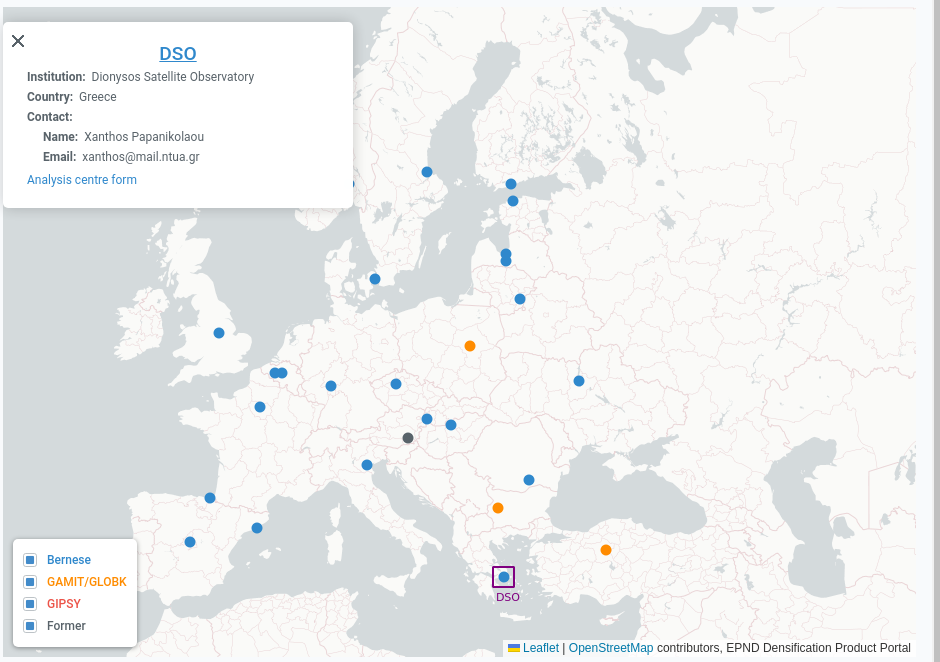
\includegraphics[width=.97\textwidth]{DSOdensmap.png}
%      \end{center}     
%    \end{column}
%  \end{columns}
%\end{frame}
%\note{}

\section{GPS/GNSS Networks in Greece}
% ------------------------------------------------------------------------------
\begin{frame}\frametitle{The Data Set}\framesubtitle{}
\vskip-1.5cm
  %To contribute to the Densification we have to establish a credible dataset
  %(network). This has proven to be rather challenging !\\
  Routine processing for precise positioning, assumes a well established, 
  credible dataset (metadata). \\
  \bigskip
  Currently we process whatever we can get our hands on \ldots\\
  Problems:
  \begin{itemize}
    \item Inhomogenous dataset (\texttt{RINEX} of various versions, raw files, etc).
    \item Various maintainers, different mentalities.
    \item Different aquisition methods/rates.
    \item No log files for mainteners with no geodetic interest (e.g. surveying companies).
    \item Wide variety of equipment (not always included in \texttt{atx} files).
  \end{itemize}
\end{frame}
\note

% ------------------------------------------------------------------------------
\begin{frame}\frametitle{Network GREECE}\framesubtitle{}
\vskip-1cm

%Network installed/maintained by \texttt{COMET}\footnote{Center for Observation and Modeling of Earthquakes, \url{http://comet.nerc.ac.uk/}} \& \texttt{NTUA}.
\begin{columns}[T] % align columns
\begin{column}{.50\textwidth}
  Network \texttt{Greece} includes the majority of the available sites ($\approx$100)
  but not all of them are (always/currently) active. Various providers but all 
  with geodetic interest \& ecquipment.

  {\small
  \begin{itemize}
    \setlength\itemsep{.1em}
    \item<pro@1-> covers all of Greece
    \item<pro@1-> different (geodetic type) equipment
    \item<pro@1-> credible time-span (early 2004 - now)
    \item<pro@1-> all free available GNSS data
    \item<con@1-> large data gaps \& inactive stations
%    \item<con@1-> needs repairing
\end{itemize}
}
\end{column}%
\hfill%
\begin{column}{.50\textwidth}
 \begin{figure}
 \begin{center}
 \vskip -.2cm
 
\includegraphics[width=.95\textwidth]{refag_greece_noref.png} %1 2.2 0 0
% \vskip-.7cm
% \caption{COMET/NTUA network.}
\href{http://dionysos.survey.ntua.gr/dsoportal/_dataanalysis/BERN52PROC/netprocinfo.php?network=greece}{->> Network GREECE}
 \label{fig:cometntua}
 \end{center}
 \end{figure}
\end{column}%
\end{columns}
%  \begin{block}{}
%    Can be used for EUREF densification ``as is''.
%  \end{block}
\end{frame}

% ------------------------------------------------------------------------------
\begin{frame}\frametitle{Network Santorini}\framesubtitle{}
\vskip-1cm
  %Network installed/maintained by \texttt{CRLab}\footnote{Rift Laboratory \url{http://webobs.crlab.eu/}}. 
  The \texttt{Santorini Volcano} ...
  \begin{columns}[T]
    \begin{column}{.4\textwidth}
      \begin{itemize}
        \item<pro@1-> credible time-span
        \item<pro@1-> only covers the Corinth Rift
        \item<con@1-> different providers (including surveying \& cadastral services)
        \item<con@1-> no log files \& equipment changes
      \end{itemize}
    \end{column}
    \begin{column}{.6\textwidth}
      \begin{figure}
      \begin{center}
        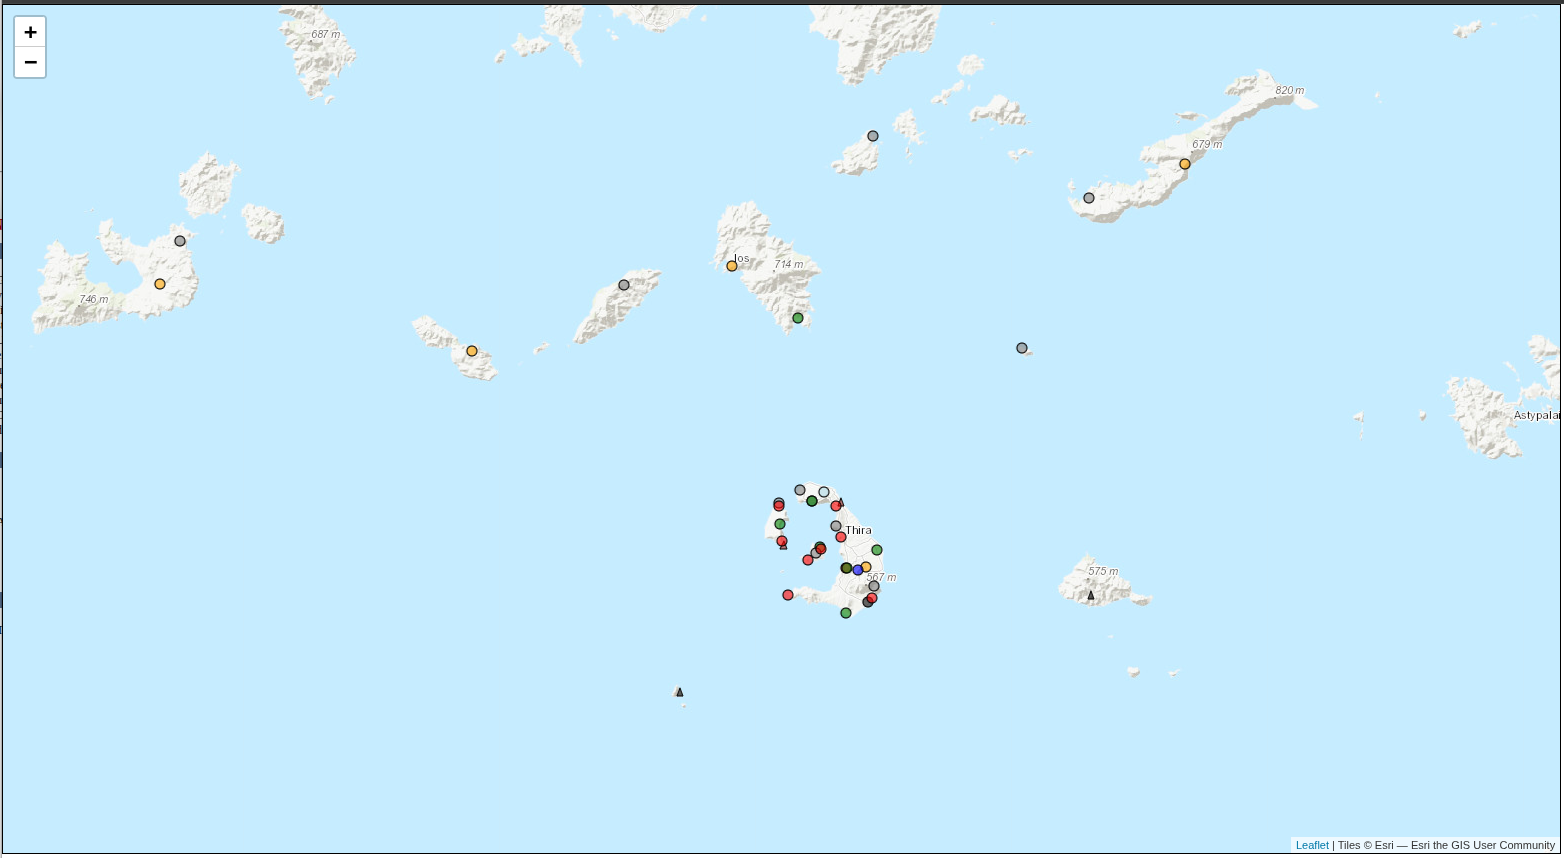
\includegraphics[trim={0cm 0cm 0cm 0cm},clip,width=.97\textwidth]{net_santo1.png}\\
        \vskip-2.5cm \hspace{-6cm}
        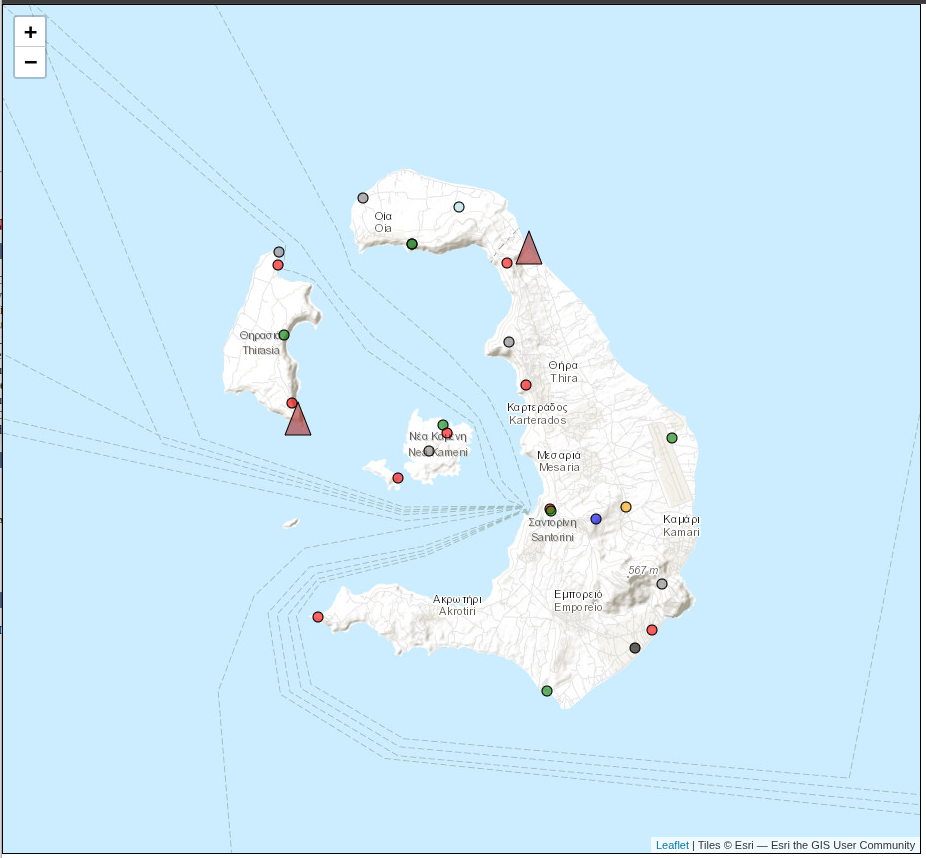
\includegraphics[trim={0cm 0cm 0cm 0cm},clip,width=.35\textwidth]{net_santo2.png}

%  \vskip .6cm
% \caption{EnCeladus network. \url{http://dionysos.survey.ntua.gr/dso/enceladus/}}
      \href{http://dionysos.survey.ntua.gr/dsoportal/_projects/supersites/santorini/}{->> Network Santorini}
     \label{fig:crlab}
     \end{center}
 \end{figure}
      
    \end{column}
  \end{columns}
\end{frame}

% ------------------------------------------------------------------------------
\begin{frame}
  \frametitle{Network HEPOS}
  \framesubtitle{}
  \label{}
 \begin{columns}[T] % align columns
	\begin{column}{.50\textwidth}
	  Network \texttt{HEPOS} 
	
	  {\small
	  \begin{itemize}
	    \setlength\itemsep{.1em}
	    \item<pro@1-> covers all of Greece
	    \item<pro@1-> homogeneous equipment
	    \item<pro@1-> credible time-span (mid 2007 - now)
	    \item<con@1-> only four years available for processing up to now
	%    \item<con@1-> needs repairing
	\end{itemize}
	}
	\begin{columns}[T]
	  \begin{column}{.5\textwidth}
	    \begin{center}
	    \vskip.5cm
	    {\small \textit{Data availability and funding from\\ Hellenic Cadastre}}
	    \end{center}
	  \end{column}
	  \begin{column}{.5\textwidth}
	     \begin{center}
	       
\includegraphics[width=.97\textwidth]{../../logos/Hellenic_cadastre.png}
	     \end{center}
	  \end{column}
	\end{columns}
	\end{column}%
	\hfill%
	\begin{column}{.50\textwidth}
	 \begin{figure}
	 \begin{center}
	 \vskip -.7cm
	 
\includegraphics[width=.95\textwidth]{hepos.png} %1 2.2 0 0
%	 \vskip-.7cm
	% \caption{COMET/NTUA network.}
	\href{http://83.212.80.177/abmaps/netmap_noref.php?network=hepos}{->> Network HEPOS}
	 \label{fig:cometntua}
	 \end{center}
	 \end{figure}
	\end{column}%
	\end{columns}
\end{frame}
\note{} 

\section{Processing}

 % ------------------------------------------------------------------------------
\begin{frame}
  \frametitle{GNSS data analysis at DSO}
  \framesubtitle{}
  \label{}
  \begin{columns}[T]
    \begin{column}{.5\textwidth}
    \textbf{GNSS data analysis}
      \begin{itemize}\setlength\itemsep{1em}
         \item Bernese v5.4 \citep{bernese_2015}
         \item PRIDE-PPPAR \citep{geng_pride_2019}
         \item GipsyX \citep{bertiger_gipsyxrtgx_2020}
       \end{itemize} 
    \textbf{Time series analysis}
    \begin{itemize}\setlength\itemsep{1em}
      \item Hector v2.1 \citep{Bos2012}
      \item Python/C++ routines
    \end{itemize}
    \end{column}
    \begin{column}{.5\textwidth}
      \textbf{Solutions}
      \begin{itemize}\setlength\itemsep{1em}
        \item Daily solution
          \begin{itemize}\setlength\itemsep{1em}
            \item Rapid solution - 1 day after
            \item Final solution - 12 days after
          \end{itemize}
        \item High-rate analysis (>1Hz)
          \begin{itemize}\setlength\itemsep{1em}
            \item data from network HEPOS - 1Hz
          \end{itemize}
      \end{itemize}
    \end{column}
  \end{columns}
  \begin{columns}[T]
    \begin{column}{.1\textwidth}
      \begin{center}
        \includegraphics[width=.7\textwidth]{logo_Bernese.png}
      \end{center}
    \end{column}
    \begin{column}{.2\textwidth}
      \begin{center}
        
\includegraphics[width=.97\textwidth]{logo_PRIDE.png}
      \end{center}      
    \end{column}
    \begin{column}{.2\textwidth}
      \begin{center}
        
\includegraphics[width=.8\textwidth]{logo_gipsyX.png}
      \end{center}      
    \end{column}
    \begin{column}{.5\textwidth}
      \begin{center}

      \end{center}      
    \end{column}    
    
  \end{columns}
\end{frame}
\note{}

% ------------------------------------------------------------------------------
\begin{frame}\frametitle{The Scheme}\framesubtitle{}
\begin{columns}[T] % align columns
\begin{column}{.35\textwidth}
\vskip-.5cm
   \footnotesize{The core tool/software is \texttt{Bernese GNSS Software v5.4}.\\
   %\medskip
   Integration with
   \begin{itemize}
    \setlength\itemsep{.5em}
     \item \textbf{PostgreSQL} database,
     \item \textbf{Python} module (product/data downloading, pre-processing, 
      driving cron jobs, etc)\\
      \url{https://github.com/DSOlab/autobern}
     \item \textbf{Time-series} analysis (integrated in routine processing on regular intervals)
     \item \textbf{Strain Rates} via StrainTool (on user demand)
   \end{itemize}}
\end{column}%
\hfill%

\begin{column}{.65\textwidth}
\vskip -.4cm
\begin{figure}
\centering
   \begin{tikzpicture}[ every annotation/.style = {draw,
                      fill = white, font = \large}]

   \path[mindmap,concept color=black!70,text=white,
     every node/.style={concept,circular drop shadow, scale=.4},
     root/.style = {concept color=black!30!red!30,
font=\normalsize\bfseries,text width=5em},
     level 1 concept/.append style={
       font=\normalsize\bfseries, sibling angle=70,text width=7.7em,
       level distance=20mm,inner sep=0pt},
     level 2 concept/.append style={font=\bfseries,level distance=15mm},
   ]

   node[root] {Bernese GNSS Software v5.4} [clockwise from=0]
     child[concept color=red!30] {
       node {pyBern Module} [clockwise from=140]
       child  [color=black!80] { node {github repo} }
       child  { node {handle PCF, BPE, flow-control} }
       child  { node {parsers\\formaters} }
       child  { node {pre-processing \& editing} }
       child  [level distance=13mm] { node {data/product downloading} }
     }
     child[concept color=blue!40] {
       node[concept] {PostrgreSQL Database} [clockwise from=-10]
       child { node[concept] {from/to .STA} }
       child { node[concept] {stations/ networks/ products} }
       child [level distance=17mm] { node[concept] {IGS log files} }
     }
     child[concept color=red!60] {
       node[concept] {Cron Jobs} [clockwise from=-40]
       child [level distance=13mm] { node[concept] {final ultra-rapid} }
       child { node[concept] {update ATX, PCV } }
       child { node[concept] {sync with AIUB} }
       child [level distance=12mm, sibling angle=70] { node[concept]
{sync with M3G} }
     }
     child[concept color=yellow!40!black!30] {
       node[concept] { Analysis } [clockwise from=220]
       child { node[concept] {Time-Series} }
       child [text width=]{ node[concept] {StrainTool} }
     }
     child[concept color=green!50] {
       node[concept] { WebPage } [clockwise from=180]
       child [level distance=12mm, text width=] { node[concept] {d3.js
plots} }
     };
\end{tikzpicture}



\label{fig:software-design}
\end{figure}

\end{column}%
\end{columns}
\end{frame}

%
%\begin{frame}\frametitle{Workflow}\framesubtitle{}
%\begin{columns}[T] % align columns
%\begin{column}{.48\textwidth}
%  \texttt{\$>ddrun.sh       --year= --doy= --session= --bern-loadgps= --campaign= --satellite-system= --solution-id= --save-dir= --analysis-center= --use-ntua-products= --append-suffix= --elevation-angle= --update= --pcv= --apply-exclude-list}
%\end{column}
%\hfill%
%\begin{column}{.48\textwidth}
%\vskip-.5cm
%  \scalebox{0.5}{
%  \smartdiagram[priority descriptive diagram]{
%    Download \texttt{RINEX} consulting \texttt{MySQL} db,
%    Download products,
%    Validate \texttt{.STA}; synchronize \texttt{/GEN},
%    Set variables in the Protocol Control File (\texttt{.PCF}),
%    Process the dataset,
%    Check for errors,
%    Save Products \& Update database records,
%    Compile Report (\texttt{json} | \texttt{html})
%}}
%\end{column}
%\end{columns}
%\end{frame}
%

%\begin{frame}\frametitle{Compliance wrt EUREF standards}\framesubtitle{}
%\vskip-1cm
%  Processing is consistent with EUREF standards (\href{http://www.epncb.oma.be/_documentation/guidelines/guidelines_analysis_centres.pdf}{Guidelines for Analysis Centres}).
%  \begin{itemize}%%[label={\checkmark}]
%    \item \texttt{SINEX} with required info/blocks,
%    \item Reference frame \texttt{\textcolor{red}{IGb14}},
%    \item \texttt{IERS} Conventions 2010,
%    \item \texttt{IGS}/\texttt{CODE} products,
%    \item ocean loading corrections (\texttt{\textcolor{red}{FES2004}}),
%    %\item atmospheric tidal loading corrections,
%    \item $3^{\circ}$ elevation cut-off angle; elevation dependent weighting,
%    \item \texttt{GMF} and/or \texttt{\textcolor{red}{VMF1}}; \texttt{Chen-Herring} gradient parameter,
%    \item amiguities fixed (length-dependent algorithm),
%    \item use \texttt{GLONASS} obs (when available)
%    \item use \texttt{ATX} files  (\textcolor{red}{epn\_14.atx}) - \textcolor{red}{individual calibrations}
%  \end{itemize}
%\end{frame}
%
%%  \begin{itemize}
%%    \item check station information file consistency (against the provided in \texttt{CODE}'s ftp)
%%    \item synchronize \texttt{GEN/} directory
%%    \item closely follow \texttt{RNX2SNX.PCF}
%%    \begin{itemize}
%%      \item variabes in PCF are set by external tools (genericity)
%%      \item skip copying/moving/removing; replace with tools that interconnect with \texttt{MySQL}
%%    \end{itemize}
%%    \item update database
%%    \item customize output (\texttt{html, json})
%%  \end{itemize}
%% \end{frame}

 % ------------------------------------------------------------------------------
\begin{frame}
  \frametitle{Switch to IGS20 -  REPRO2026}
  \framesubtitle{}
  \label{}
  \vspace*{-.5cm}
%  $\Rightarrow$ New release Bernese GNSS Software \textcolor{blue}{v5.4}\\[1em]
%  New values on processing options:
  \begin{itemize}\setlength\itemsep{.2em}
    \item Reference frame \texttt{\textcolor{blue}{IGS20 > IGb20 > IGc20}}
    \item Oceans loading corrections (\texttt{\textcolor{blue}{NTUA\_FES2014b}})
    \item \texttt{\textcolor{blue}{VMF3}} for tropospheric modeling
    \item \texttt{ATX} file: \texttt{\textcolor{blue}{igs20.atx}}
    \item \textcolor{blue}{Long filename of products} according to new IGS convention
  \end{itemize}
  ~\\[.2em]
  \begin{center}
    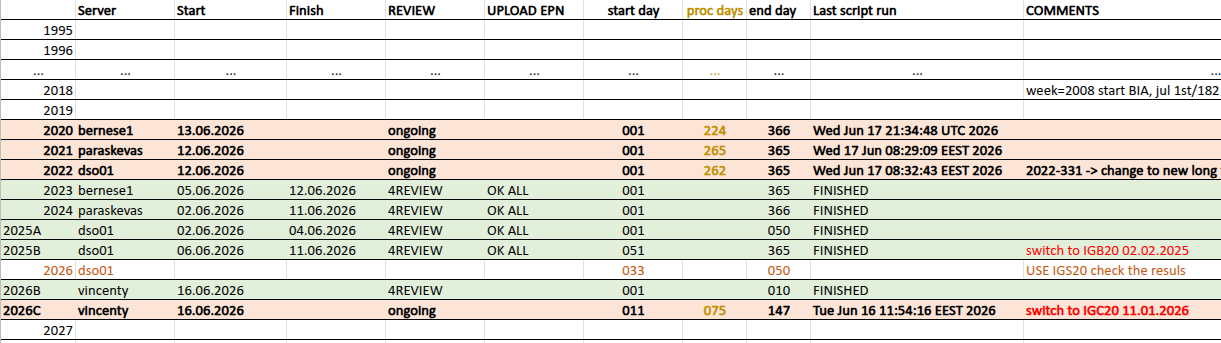
\includegraphics[width=.97\textwidth]{repro26_status.png}
  \end{center}
%  $\Rightarrow$  
%  $\Rightarrow$ Reprocess all available data from late '90s up to now
\end{frame}
\note{}

% % ------------------------------------------------------------------------------
%\begin{frame}
%  \frametitle{REPRO26 status}
%  \framesubtitle{}
%  \label{}
%  \begin{center}
%    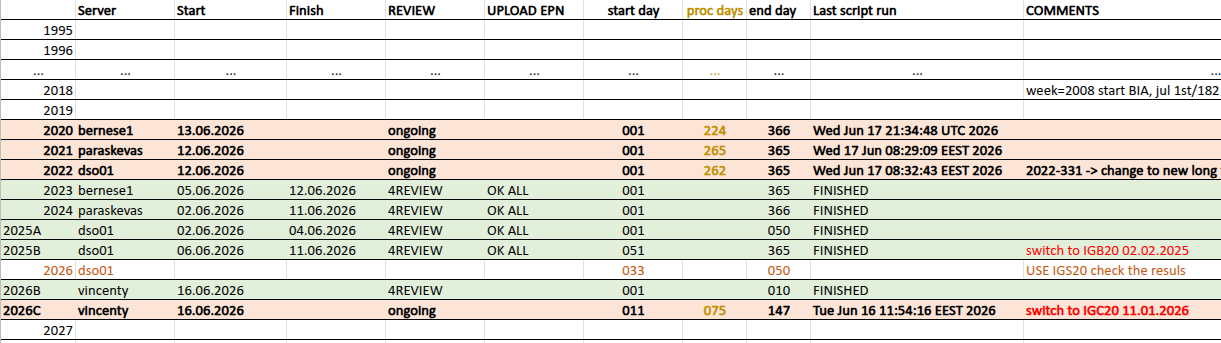
\includegraphics[width=.97\textwidth]{repro26_status.png}
%  \end{center}
%\end{frame}
%\note{}

 % ------------------------------------------------------------------------------
\begin{frame}
  \frametitle{Turn to new DB}
  \framesubtitle{}
  \label{}
  \begin{center}
    \vskip-1cm
    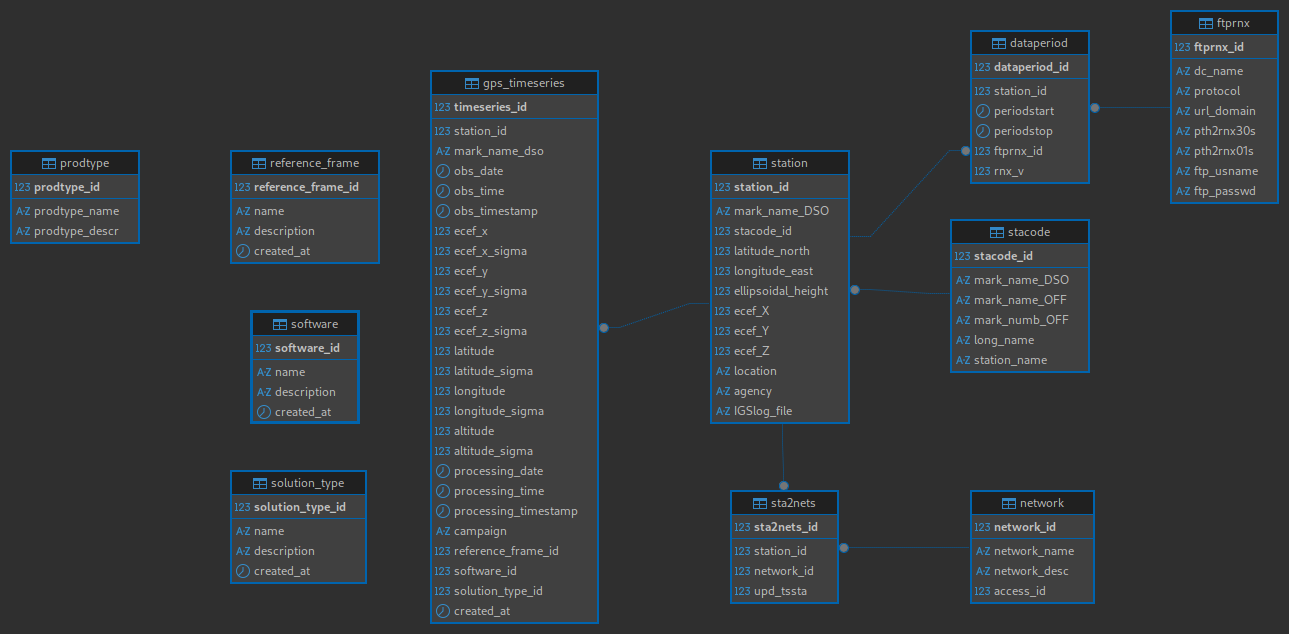
\includegraphics[width=.9\textwidth]{procsta_public_diagram.png}
  \end{center}
\end{frame}
\note{
Για την εφαρμογή επιλέχθηκε το PostgreSQL ως σύστημα διαχείρισης βάσης δεδομένων.
Κριτήρια επιλογής:
    \begin{itemize}
        \item Ελεύθερου και ανοικτού κώδικα (FOSS).
        \item Αξιόπιστη διαχείριση μεγάλου όγκου δεδομένων.
        \item Ισχυρή υποστήριξη χρονικών τύπων και σύνθετων SQL ερωτημάτων.
        \item Ευρεία χρήση σε επιστημονικές και εμπορικές εφαρμογές.
        \item Υποστήριξη επεκτάσεων όπως PostGIS για χωρικά δεδομένα.
    \end{itemize}
Σε σύγκριση με το MySQL, προσφέρει μεγαλύτερη ευελιξία σε τύπους δεδομένων και επεκτασιμότητα.
}

% % ------------------------------------------------------------------------------
%\begin{frame}
%  \frametitle{Flowchart}
%  \framesubtitle{}
%  \label{}
%\resizebox{0.95\textwidth}{!}{%
%\begin{tikzpicture}[
%  box/.style={
%    rectangle, draw, rounded corners=4pt,
%    align=center, font=\scriptsize,
%    minimum width=3.9cm, minimum height=0.95cm
%  }
%]
%
%% Nodes (simple coordinates that always work)
%\node[box, fill=blue!15]   (ui)     at (0,0)   {User/Frontend};
%\node[box, fill=gray!15]   (params) at (4.4,0) {Parameters\\$[t_{start},t_{end}]$\\solution\\frame};
%\node[box, fill=green!15]  (api)    at (8.8,0) {Processing Part};
%
%\node[box, fill=orange!20] (db)     at (8.8,-2.2) {PostgreSQL};
%\node[box, fill=blue!15]   (viz)    at (3,-2.2) {Diagrams};
%\node[box, fill=red!50] (bpe)     at (8.8,-4.2) {BPE54};
%
%% Arrows exactly as requested
%\draw[->, thick] (ui) -- (params);
%\draw[->, thick] (params) -- (api);
%
%\draw[->, thick] (api) -- node[right]{SQL} (db);
%\draw[->, thick] (db) -- node[left]{Records} (api);
%
%\draw[->, thick] (api) -- (viz);
%
%\draw[<->, thick] (db) -- (bpe);
%
%\end{tikzpicture}%
%}
%
%\end{frame}
%\note{}

 % ------------------------------------------------------------------------------
\begin{frame}
  \frametitle{Platform flowchart}
  \framesubtitle{}
  \label{}
\resizebox{0.94\textwidth}{!}{%
\begin{tikzpicture}[
    font=\small,
    >=Latex,
    node distance=2.5cm,
    box/.style={
        draw,
        rounded corners=8pt,
        minimum width=4cm,
        minimum height=1.2cm,
        align=center,
        thick,
        drop shadow,
        text width=3.6cm
    }
]

% Nodes
\node[box,
      top color=blue!20,
      bottom color=blue!5] (ui)
      at (0,0)
      {\textbf{User Interface}\\Frontend};

\node[box,
      top color=violet!20,
      bottom color=violet!5] (params)
      at (5,0)
      {\textbf{Parameters}\\
       $[t_{start},t_{end}]$\\
       Solution Type\\
       Reference Frame};

\node[box,
      top color=green!25,
      bottom color=green!5] (api)
      at (10,0)
      {\textbf{Timeseries analysis}};

\node[
  cylinder,
  shape border rotate=90,
  aspect=0.25,
  draw,
  thick,
  fill=orange!20,
  minimum height=1.4cm,
  minimum width=2.5cm,
  align=center,
  drop shadow
] (db) at (10,-2.8) {\textbf{PostgreSQL}};

\node[box,
      top color=cyan!25,
      bottom color=cyan!5]
      (viz)
      at (3,-2.5)
      {\textbf{Visualization}\\Charts \& Analytics};

\node[box,
      top color=red!30,
      bottom color=red!10]
      (bpe)
      at (10,-5.2)
      {\textbf{BPE54}\\GNSS Data Source};

% Flow arrows
\draw[->, ultra thick, blue!70]
    (ui) -- (params);

\draw[->, ultra thick, violet!70]
    (params) -- (api);

\draw[->, ultra thick, green!70]
    (api) -- node[right,font=\footnotesize]{SQL} (db);

\draw[->, ultra thick, green!70]
    (db) -- node[left,font=\footnotesize]{Records} (api);

\draw[->, ultra thick, cyan!70]
    (api) to[bend left=15] (viz);

\draw[<->, ultra thick, red!70]
    (db) -- (bpe);

\end{tikzpicture}
}
\end{frame}
\note{}

 % ------------------------------------------------------------------------------
\begin{frame}
  \frametitle{Presentation Layer - Main Application Screen}
  \framesubtitle{}
  \label{}
  \vspace{-.8cm}
  \begin{columns}[T]
    \begin{column}{.45\textwidth}
      \begin{itemize}

				\item User entry point to the application.
				
				\vspace{0.25cm}
				
				\item Selection of basic parameters:
				\begin{itemize}
				\setbeamertemplate{itemize subitem}{$\diamond$}
				\item GNSS station
				\item Solution type
				\item Reference frame
				\end{itemize}
				
				\vspace{0.35cm}
				
				\item Filtering and reordering capability
				
      \end{itemize}
      \textbf{Live app (beta version):}
      \begin{center}
      \vskip-.3cm
        
\includegraphics[width=.55\textwidth]{server_8585_qr}
      \end{center}
    \end{column}
    \begin{column}{.55\textwidth}
      \begin{center}
      \vskip-.5cm
        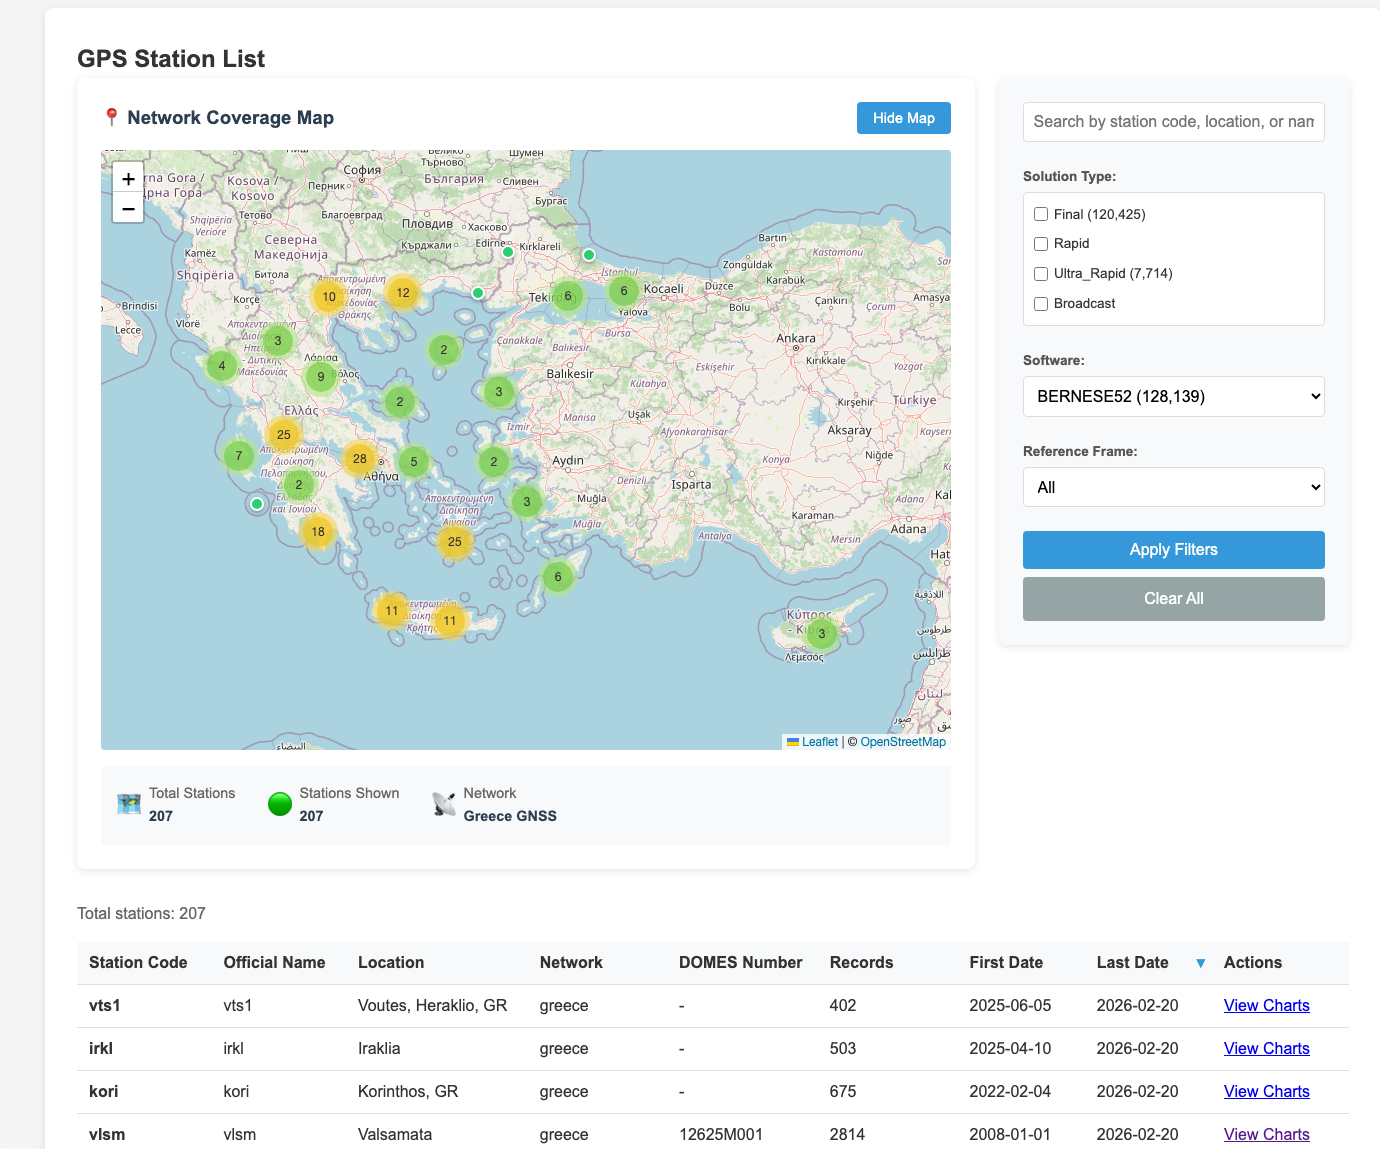
\includegraphics[width=.97\textwidth]{ui_home.png}\\
        \url{http://83.212.80.177:8585/}
      \end{center}
    \end{column}
  \end{columns}

\end{frame}
\note{}



\section{Results \& Outputs}

{
\usebackgroundtemplate{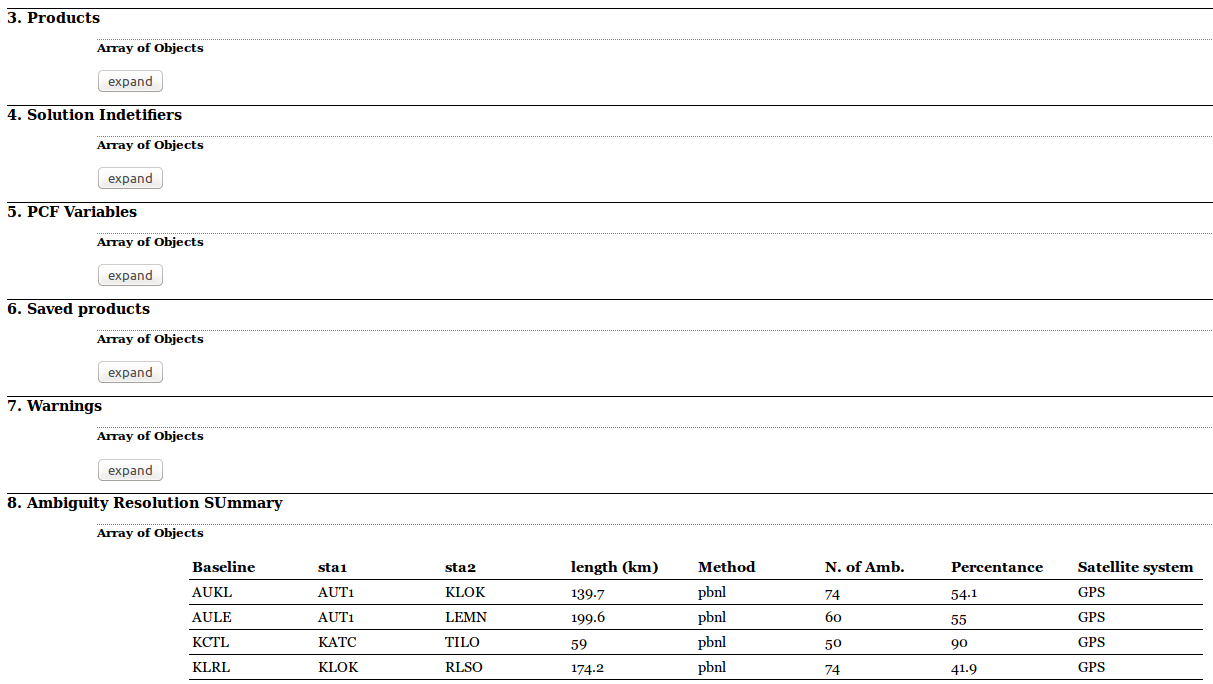
\includegraphics[height=.9\paperheight,width=.9\paperwidth]{jsonprint.png}}
\vskip-1.5cm
\begin{frame}\frametitle{Results \& Output}\framesubtitle{}
\begin{center}
\vskip -1.6cm
\begin{tikzpicture}
  \node (img1) {\shadowbox{\color{black!35}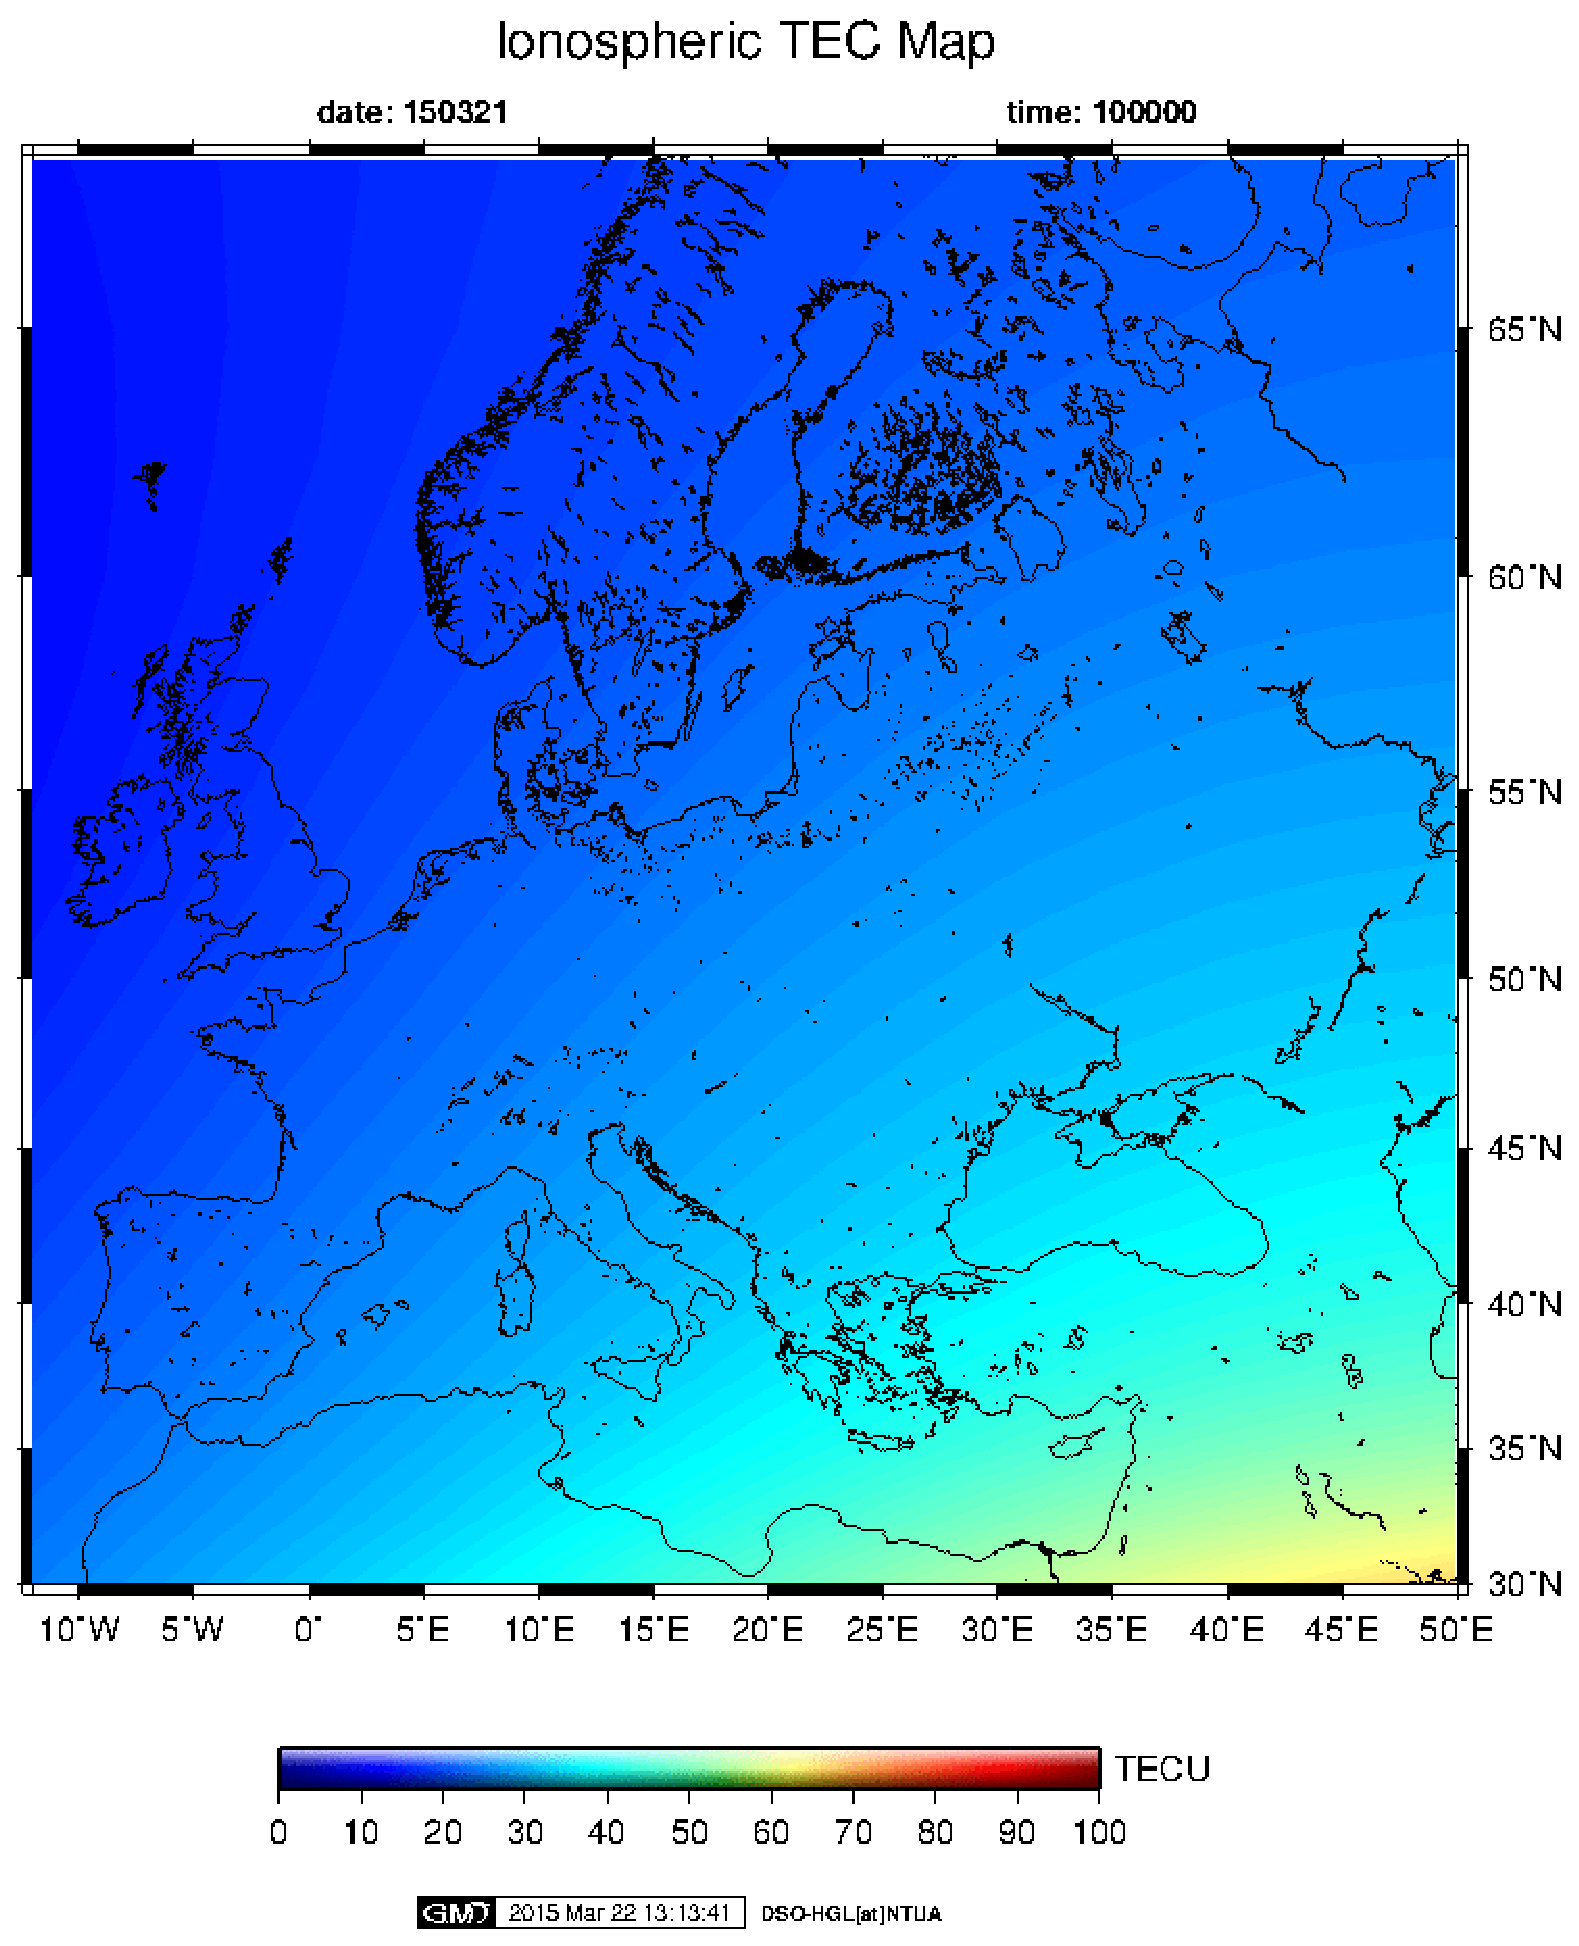
\includegraphics[height=4cm]{iono.eps}}};
%   \pause
  \node (img2) at (img1.north east) [yshift=-1cm,xshift=2.7cm] {\shadowbox{\color{black!35}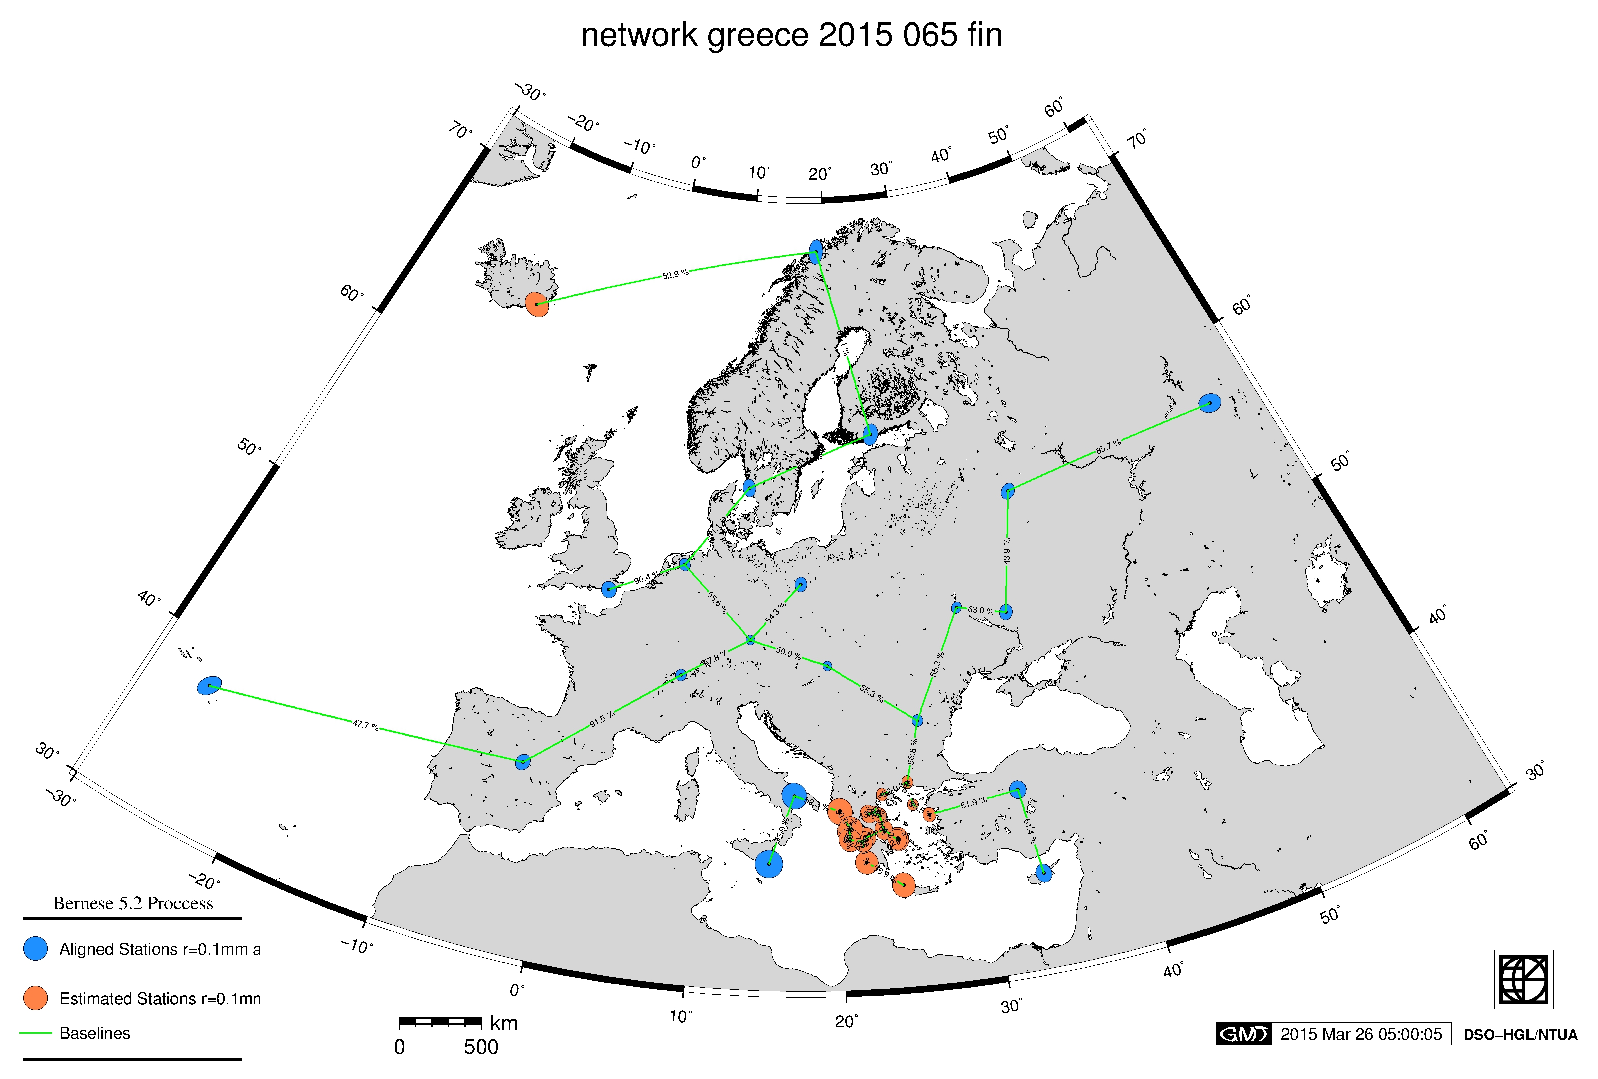
\includegraphics[height=2cm]{baseline.eps}}};
%   \pause
  \node (img3) at (img2.south) [yshift=-1.5cm,xshift=-.5cm] {\shadowbox{\color{black!35}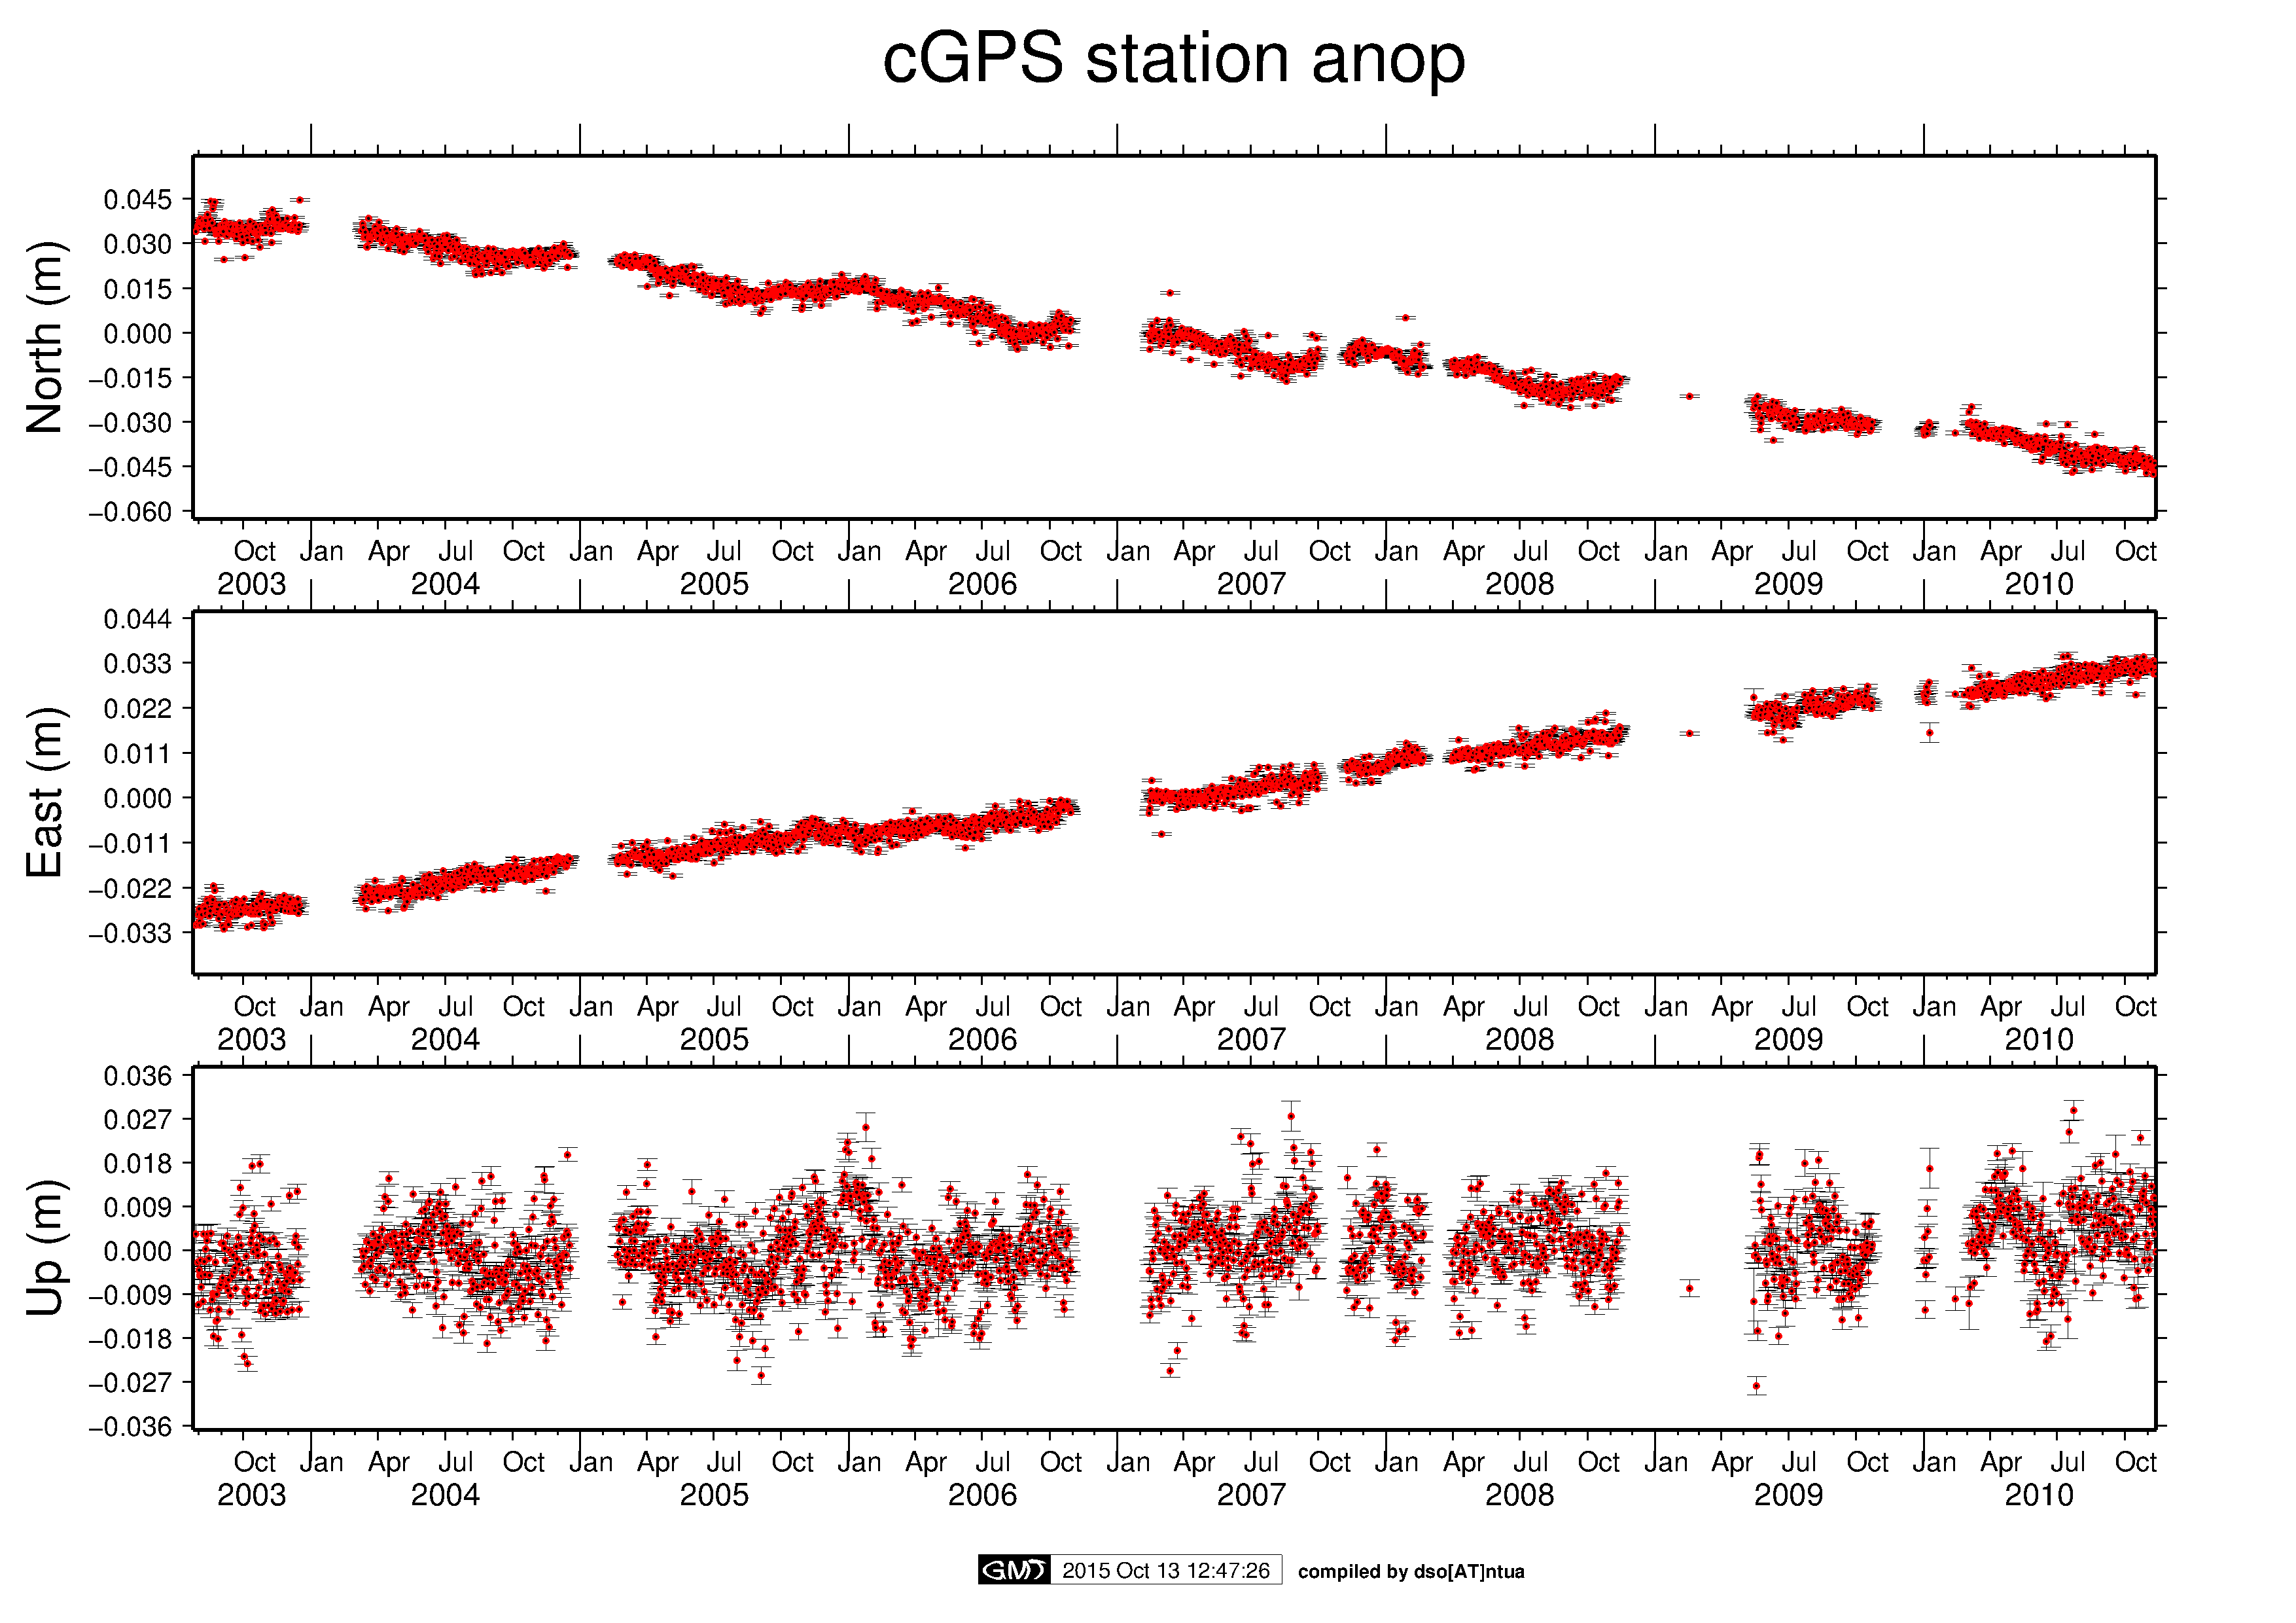
\includegraphics[height=2.6cm]{anop-raw.png}}};
%   \pause
%   \node (img4) at (img2.south west) [yshift=2cm] {\includegraphics[height=4cm]{img/dsoprint.png}};
\end{tikzpicture}
\end{center}
\end{frame}
}

 % ------------------------------------------------------------------------------
\begin{frame}
  \frametitle{Online results}
  \framesubtitle{}
  \label{}
  \begin{columns}[T]
    \begin{column}{.33\textwidth}
      \begin{center}
        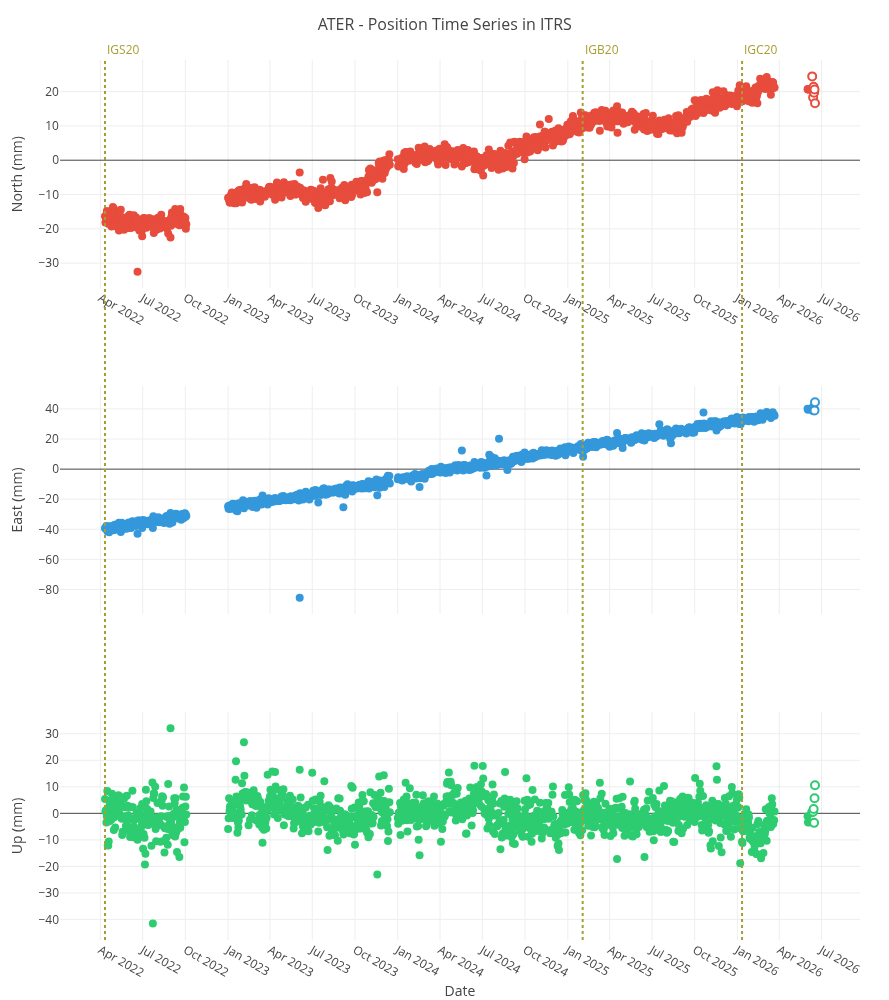
\includegraphics[width=.97\textwidth]{ater_ts.png}
      \end{center}
    \end{column}
    \begin{column}{.33\textwidth}
      \begin{center}
        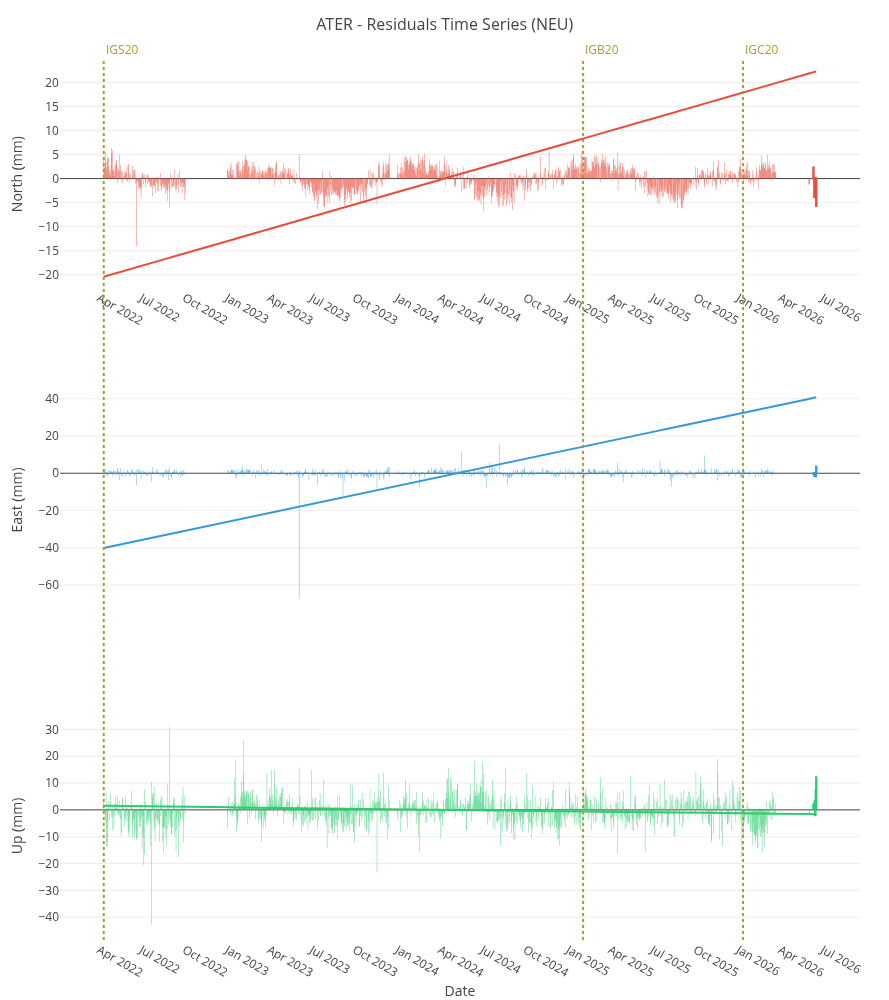
\includegraphics[width=.97\textwidth]{ater_res.png}
      \end{center}
    \end{column}
%    \begin{column}{.25\textwidth}
%      \begin{center}
%        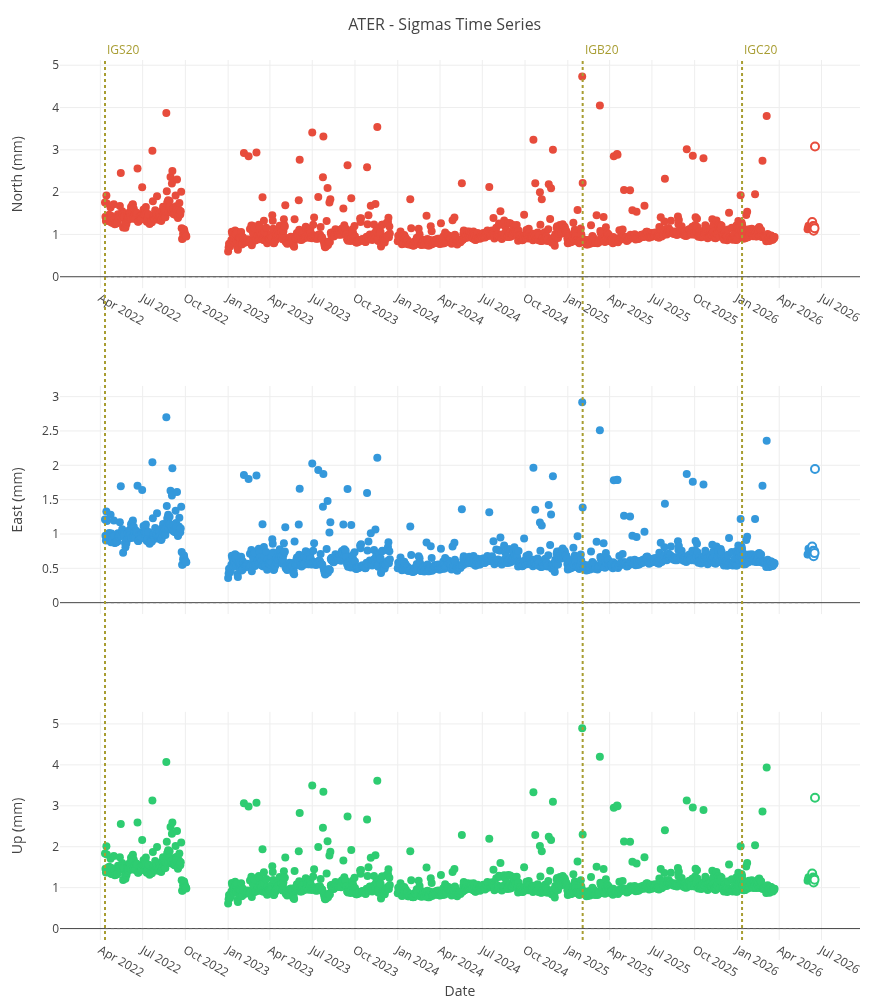
\includegraphics[width=.97\textwidth]{ater_sigma.png}
%      \end{center}
%    \end{column}
    \begin{column}{.33\textwidth}
      \begin{center}
        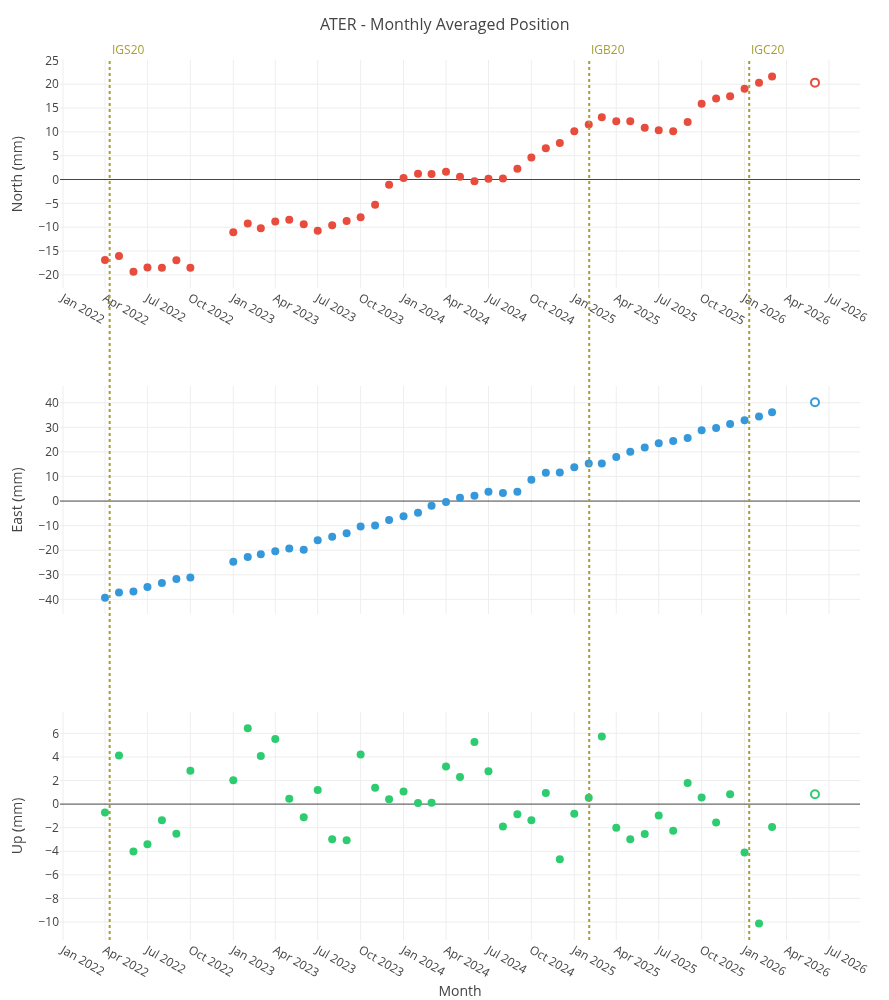
\includegraphics[width=.97\textwidth]{ater_monthly.png}
      \end{center}
    \end{column}
  \end{columns}
\end{frame}
\note{}



 % ------------------------------------------------------------------------------
\begin{frame}
  \frametitle{Time series analysis}
  \framesubtitle{Linear+Seasonal+PSD}
  \label{}
\begin{align*}
    y(\delta t) &= A \delta t + B + C_1 \sin(\omega_1 \delta t) + D_1 \cos(\omega_1 \delta t)
    + C_2 \sin(\omega_2 \delta t) + D_2 \cos(\omega_2 \delta t) \\
   & + \sum_{k=1}^{n} J_k H(t - t_k)
    + \sum_{i=1}^{n} A_i' \log\!\left(1 + \frac{\delta t}{T_i'}\right)
    + \sum_{j=1}^{n} A_j \left(1 - e^{-\frac{\delta t}{\tau_j}}\right)
\end{align*}

\end{frame}
\note{}

 % ------------------------------------------------------------------------------
\begin{frame}
  \frametitle{Preliminary Results in Greece}
  \framesubtitle{}
  \label{}
  \vspace*{-1cm}
  \begin{columns}[T]
    \begin{column}{.33\textwidth}
      \begin{center}
        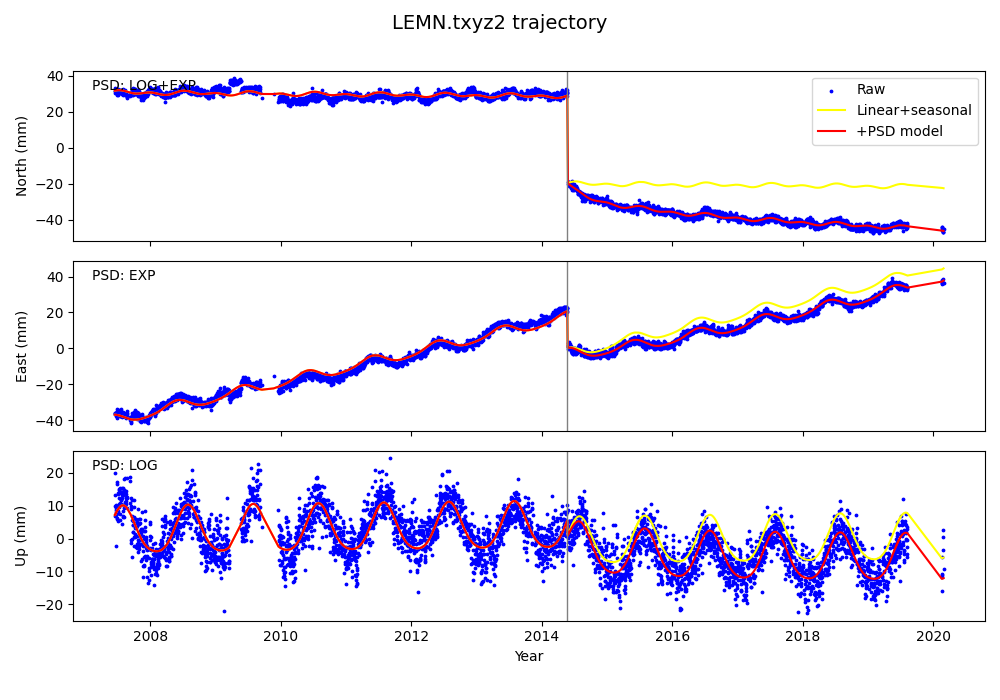
\includegraphics[width=.97\textwidth]{LEMN_ts.png}\\
        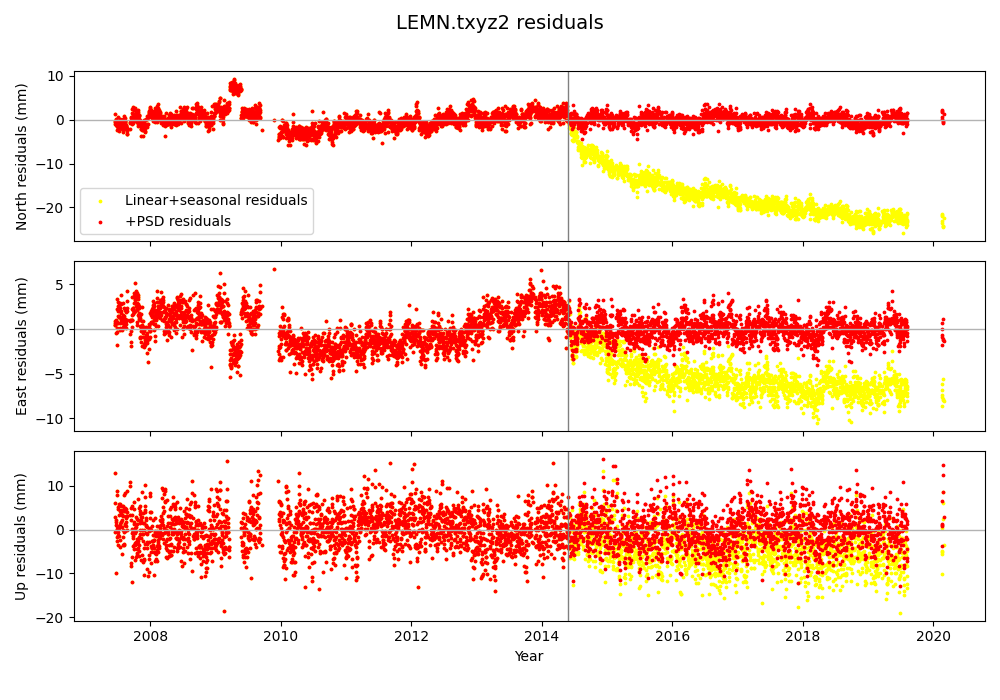
\includegraphics[width=.97\textwidth]{LEMN_res.png} 
      \end{center}
    \end{column}
    \begin{column}{.33\textwidth}
      \begin{center}
        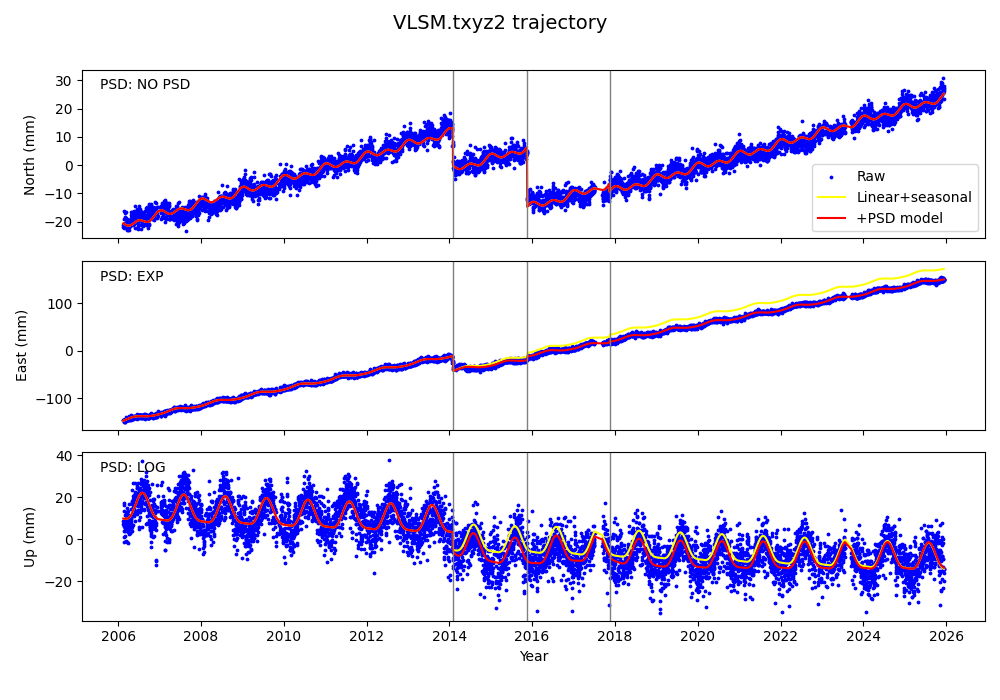
\includegraphics[width=.97\textwidth]{VLSM_ts.png}\\
        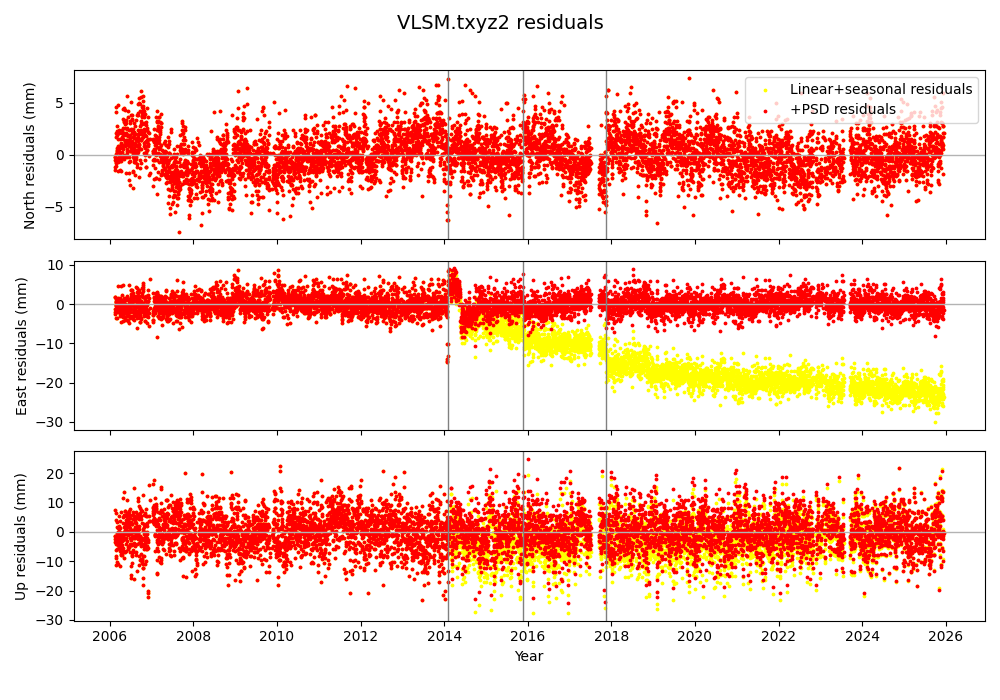
\includegraphics[width=.97\textwidth]{VLSM_res.png} 
      \end{center}      
    \end{column}
     \begin{column}{.33\textwidth}
      \begin{center}
        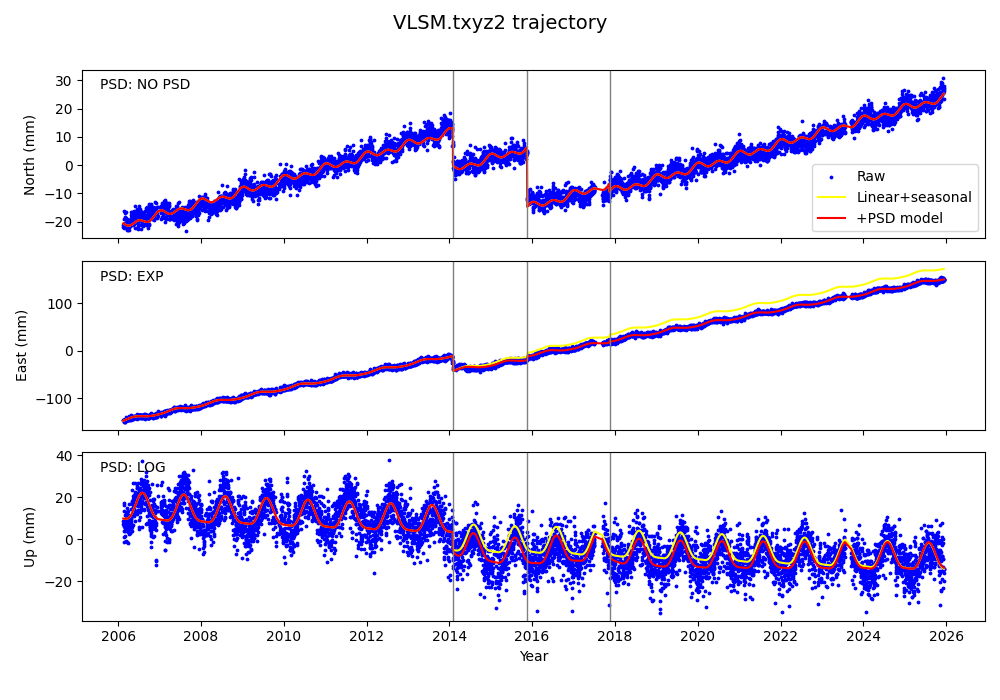
\includegraphics[width=.97\textwidth]{VLSM_ts.png}\\
        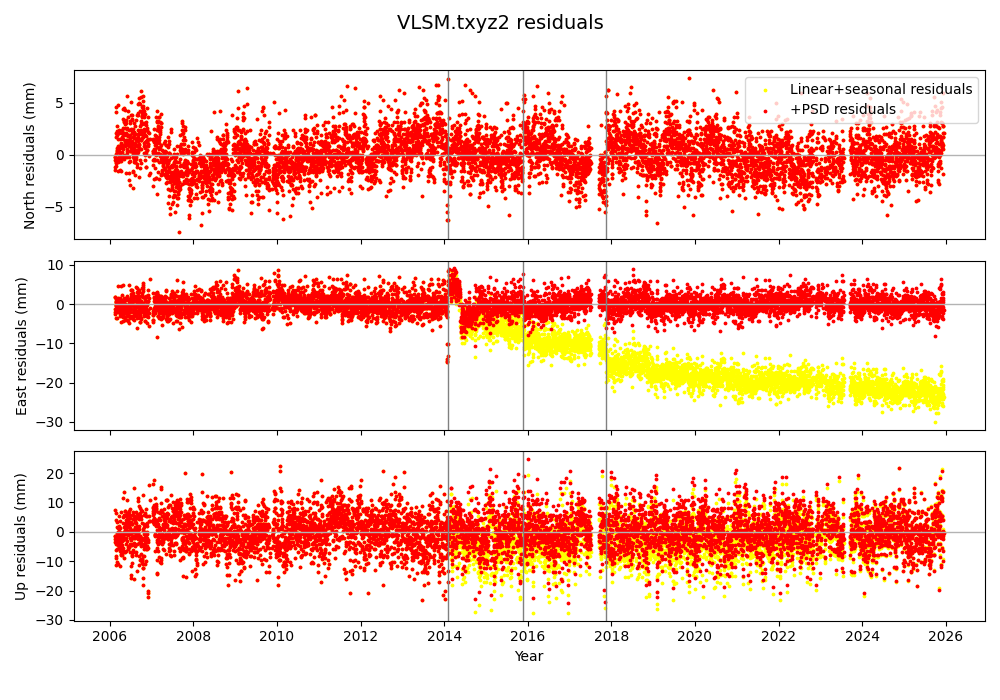
\includegraphics[width=.97\textwidth]{VLSM_res.png} 
      \end{center}      
    \end{column}
  \end{columns}

\end{frame}
\note{}


 % ------------------------------------------------------------------------------
\begin{frame}
  \frametitle{Specific case - Santorini}
  \framesubtitle{}
  \label{}
  \vskip-1cm
  \begin{columns}[T]
%    \begin{column}{.33\textwidth}
%    \vskip.5cm
%    Estimate velocity changes in Santorini station:
%    \begin{table}[H]{\small
%    \begin{center}
%    \begin{tabular*}{.97\linewidth}{@{\extracolsep{\fill}} l c c}
%      \toprule
%        comp & < $\sim$2013 & > $\sim$ 2013\\
%             & \multicolumn{2}{c}{(mm/yr)}\\
%      \midrule
%        north & -30.1 & -17.5 \\
%        east  &  31.3 & 7.0 \\
%        up    &  17.2 & 2.1 \\
%      \bottomrule
%    \end{tabular*}
%    \end{center}}
%    \end{table}
%
%
%    \end{column}
    \begin{column}{.22\textwidth}
      \begin{center}
      \textbf{SNTR}\\
         
\includegraphics[width=.97\textwidth]{sntr-mod.png}\\
       \end{center} 
    \end{column}
    \begin{column}{.22\textwidth}
      \begin{center}
      \textbf{048A}\\
         
\includegraphics[width=.97\textwidth]{048a-mod.png}\\
       \end{center} 
    \end{column}
    \begin{column}{.22\textwidth}
      \begin{center}
      \textbf{SNT2}\\
         
\includegraphics[width=.97\textwidth]{snt2-mod.png}\\
       \end{center} 
    \end{column}
    \begin{column}{.32\textwidth}
      \begin{center}
      \vspace*{-.3cm}
         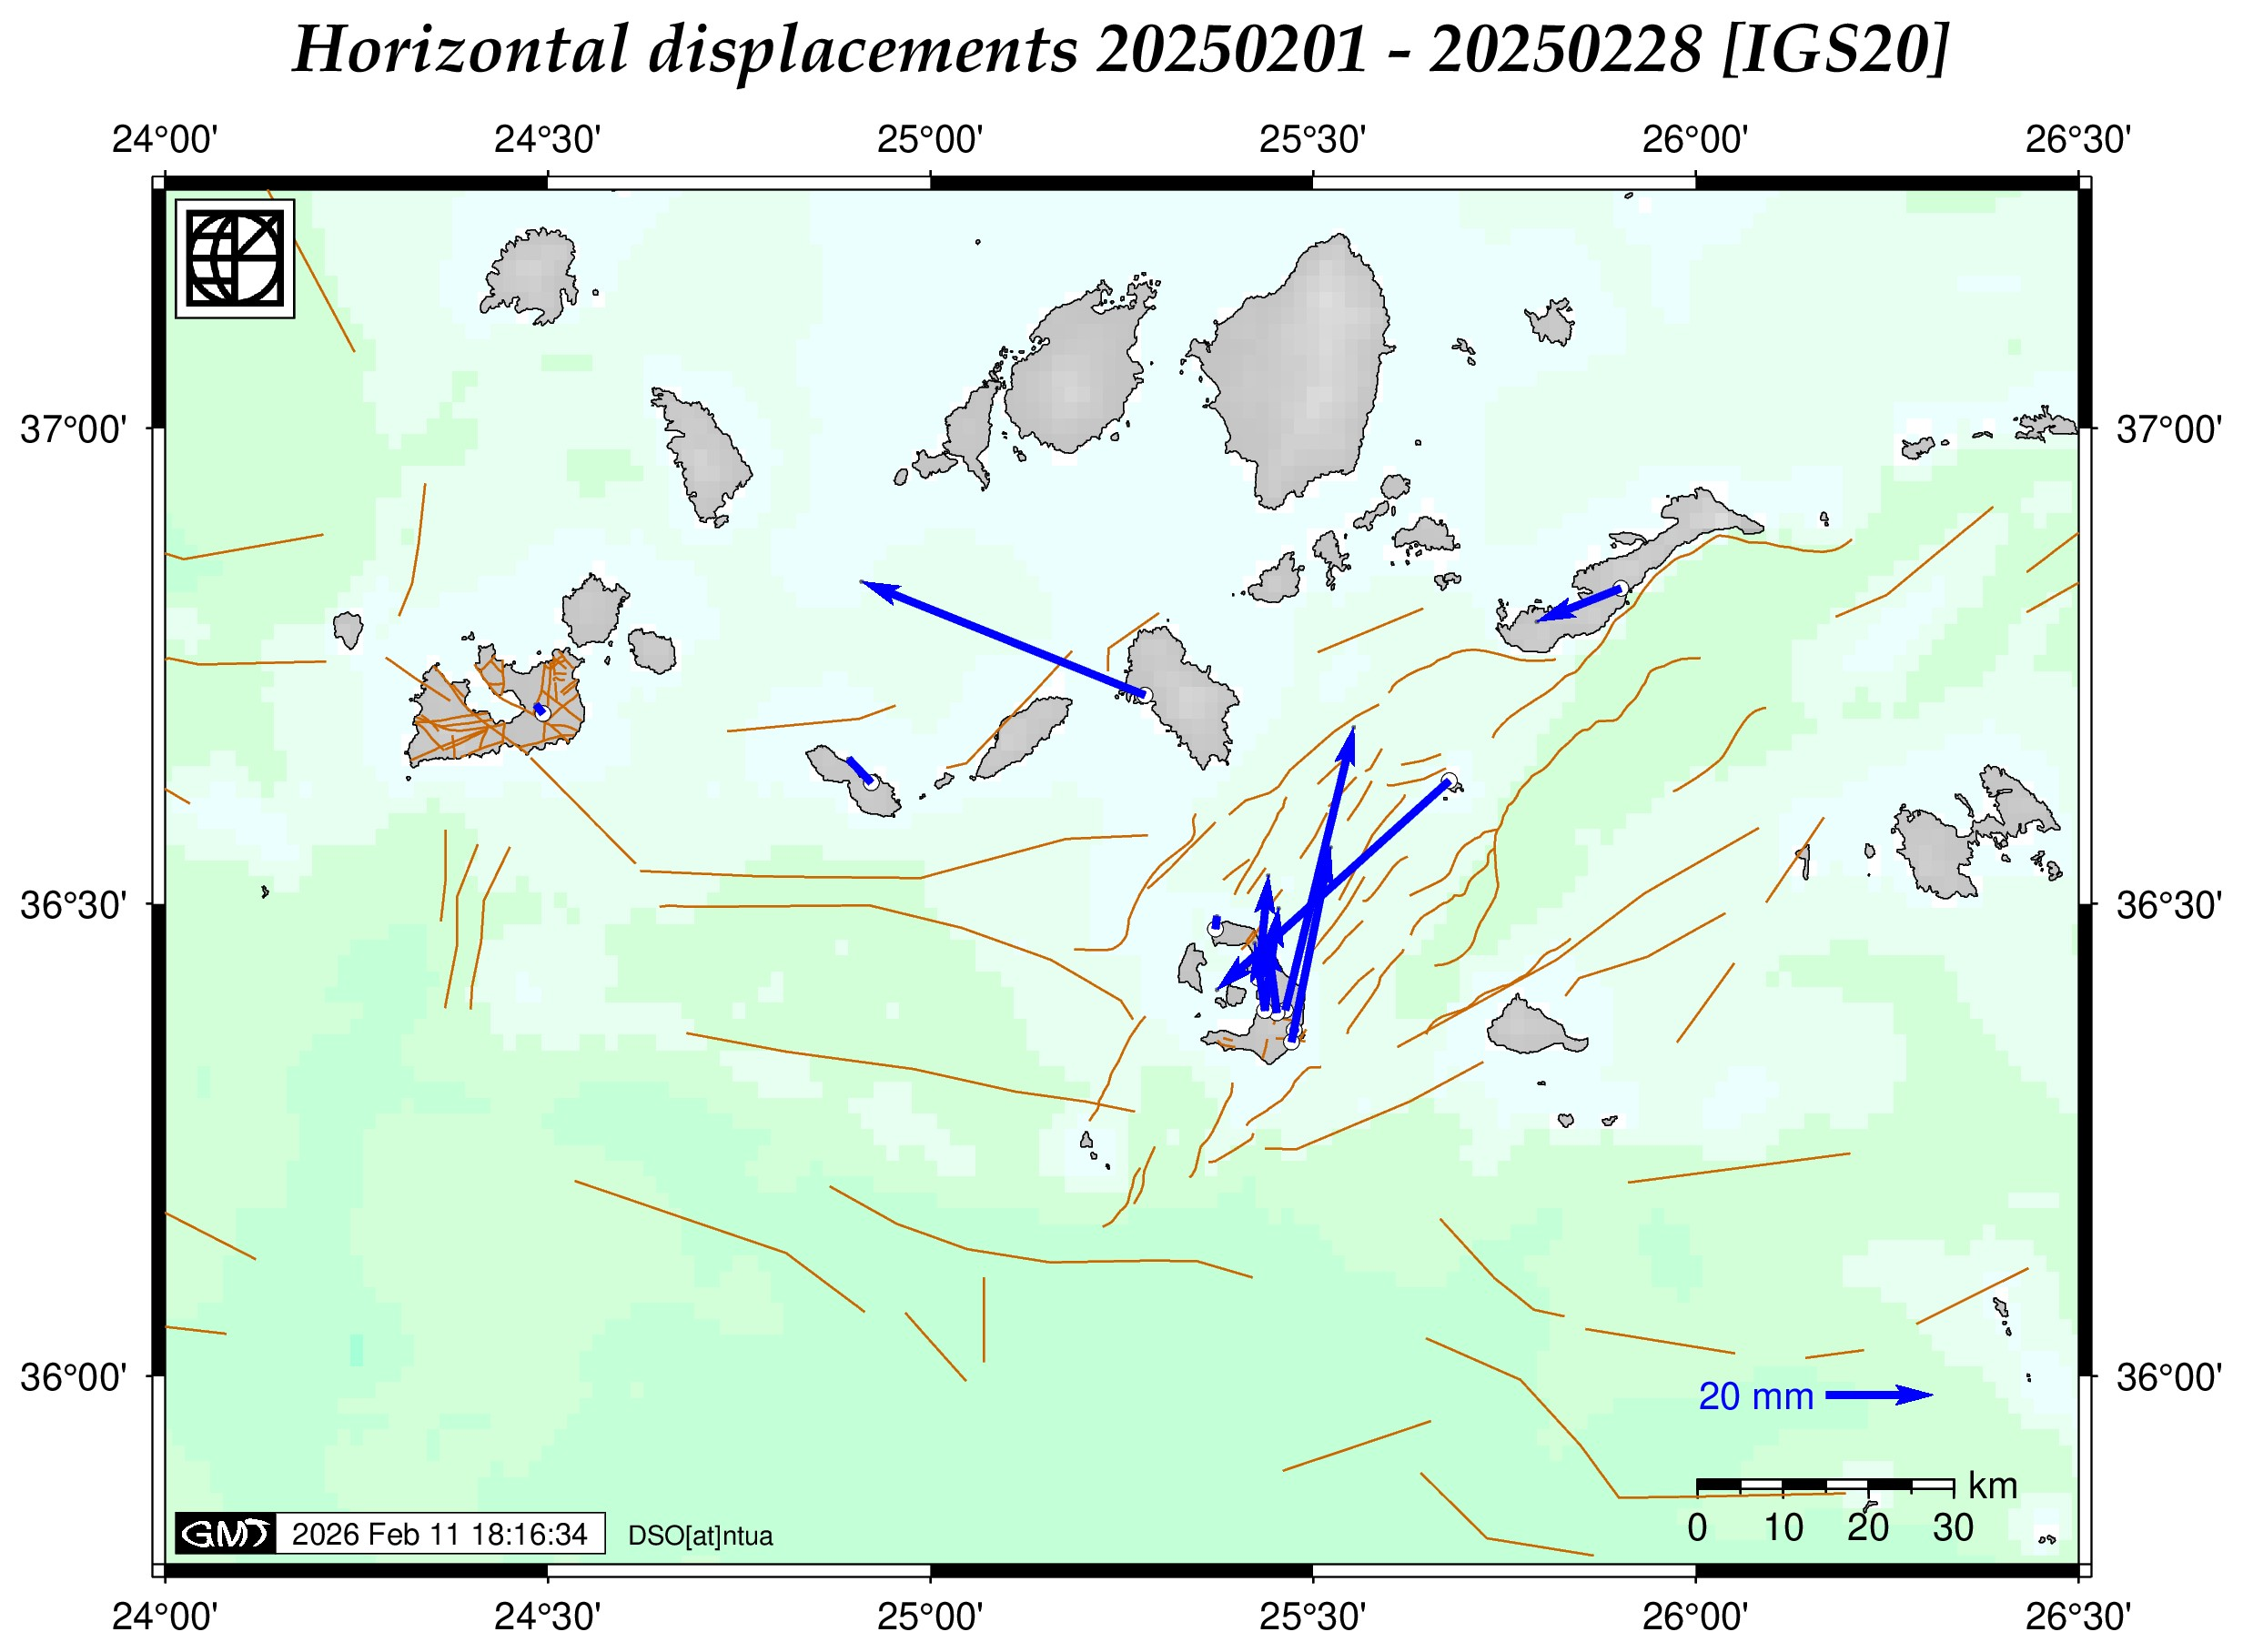
\includegraphics[width=.97\textwidth]{gnss_20250201_20250228_hdisp.jpg}\\
         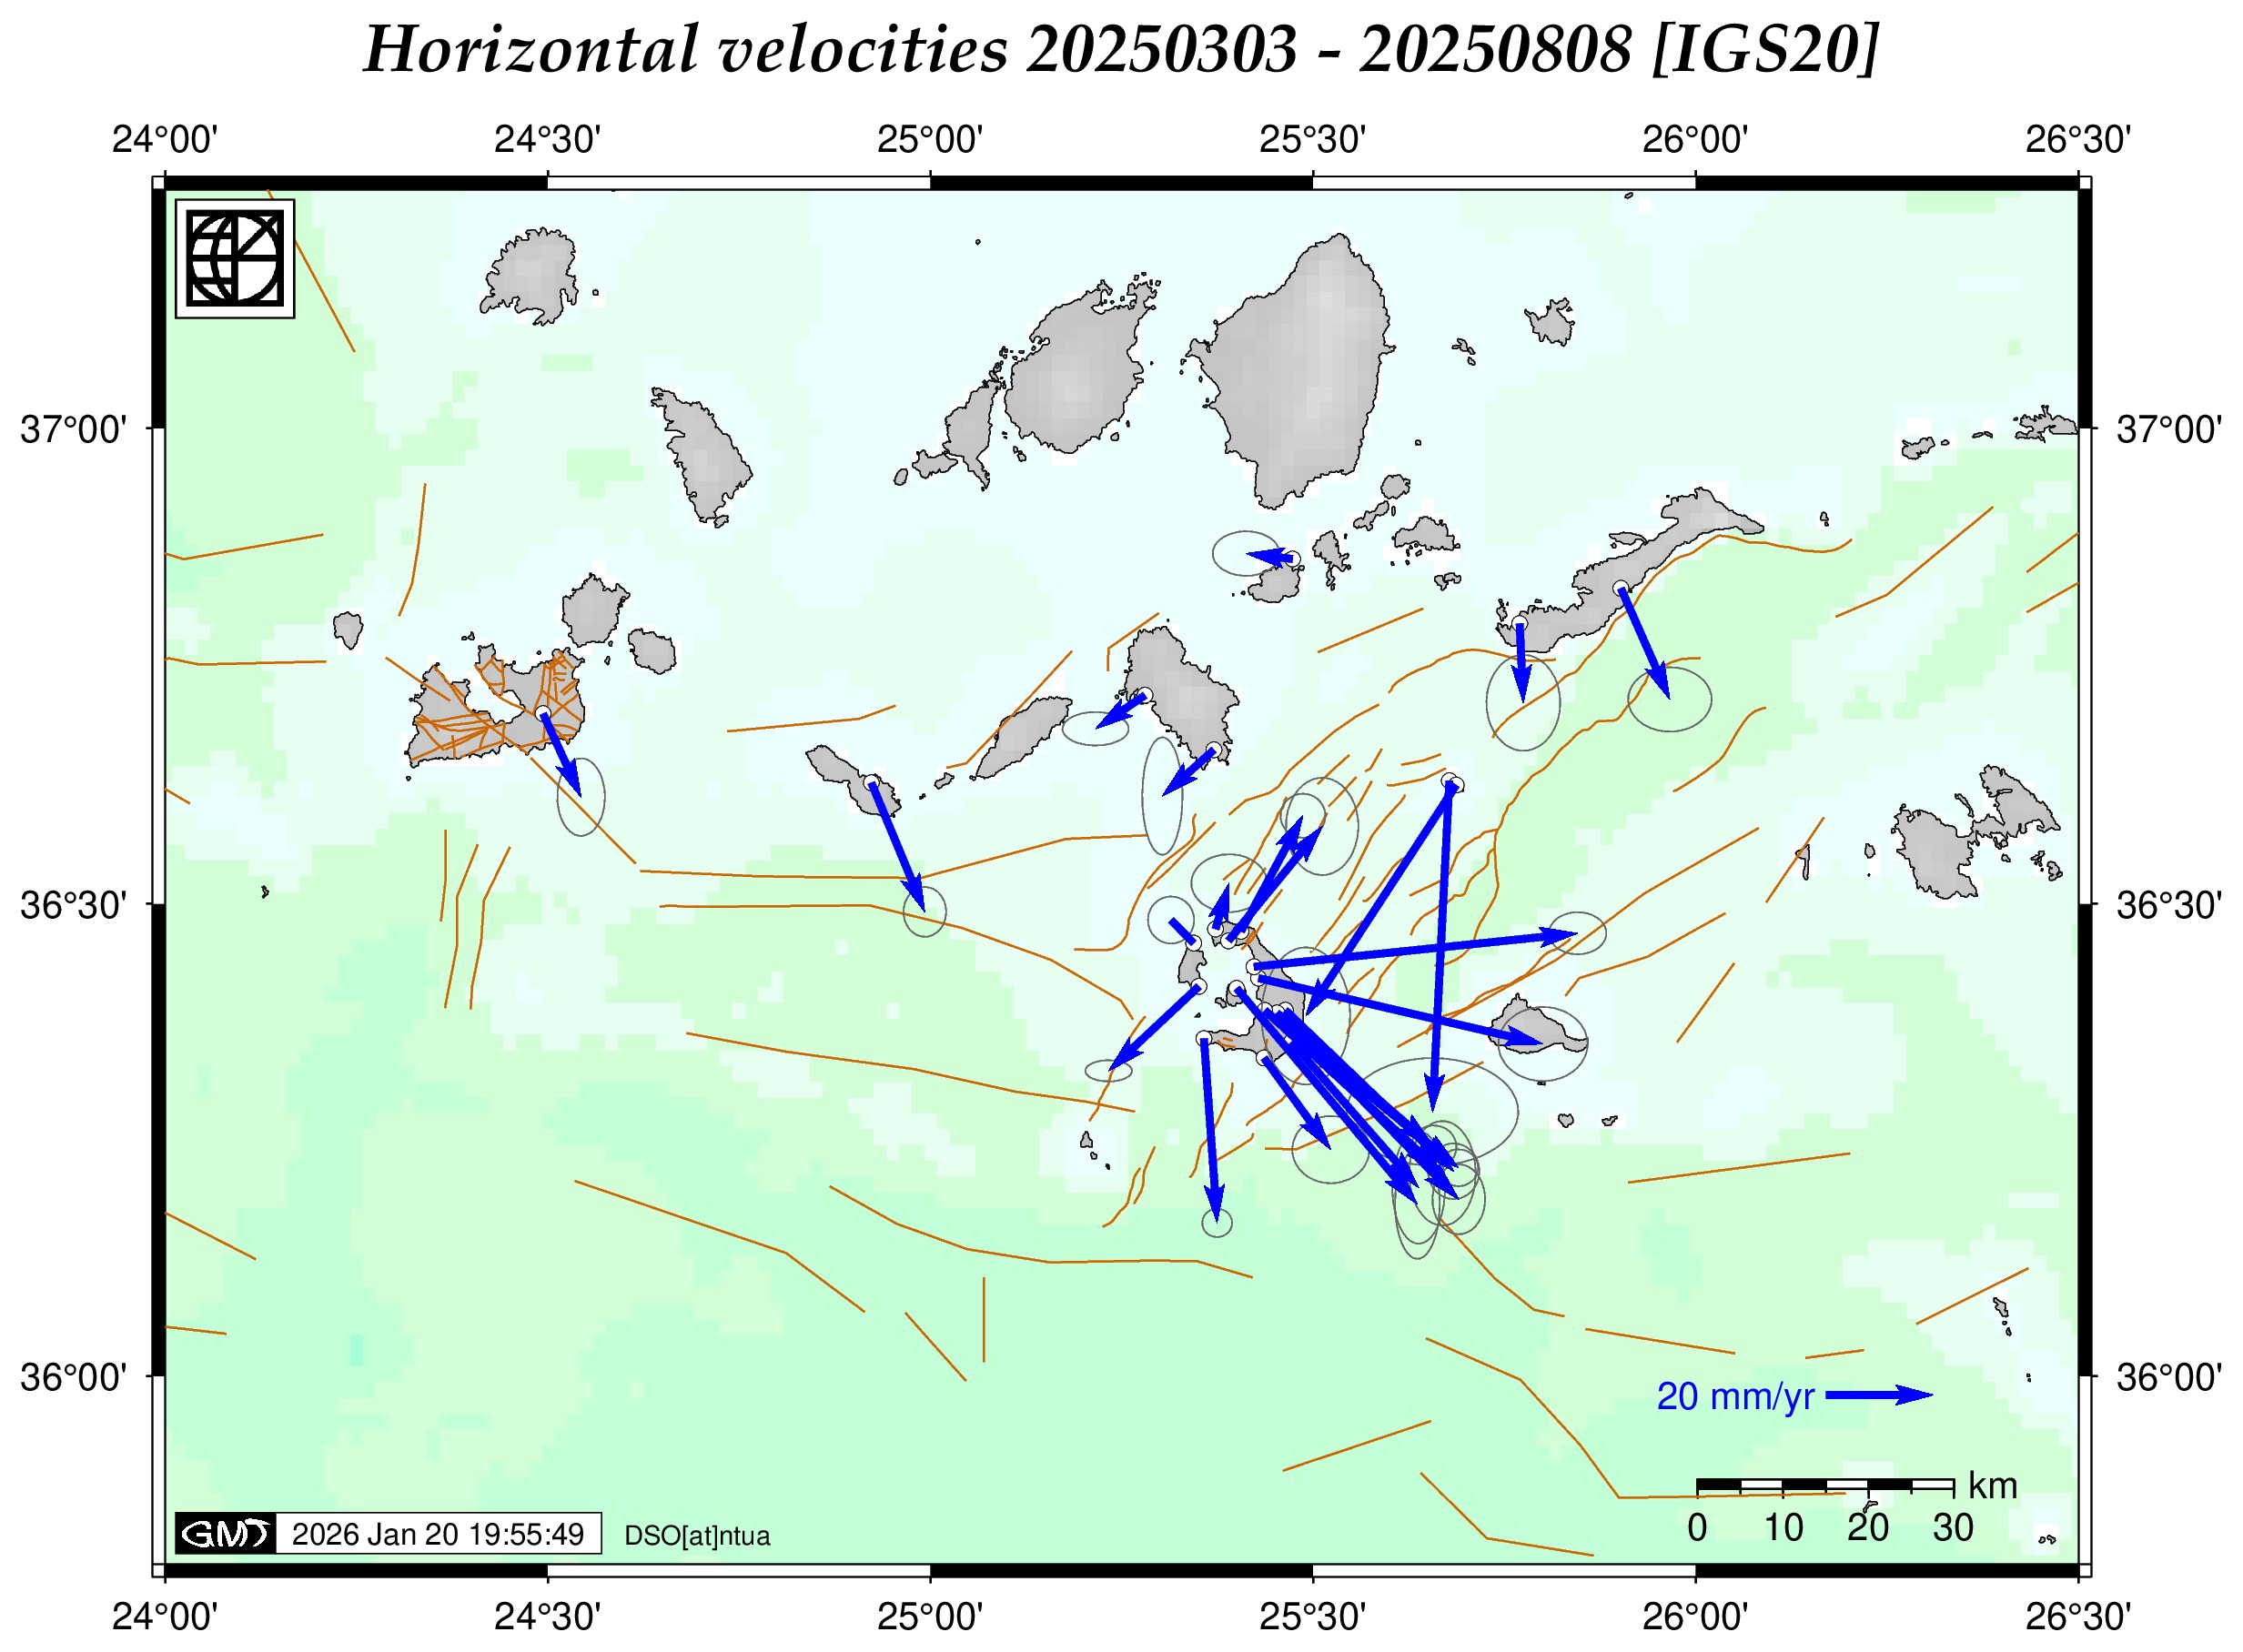
\includegraphics[width=.97\textwidth]{cycl_20250303_20250808_vhorlin.jpg}
       \end{center} 
    \end{column}
  \end{columns}
\end{frame}
\note{}



% % ------------------------------------------------------------------------------
%\begin{frame}
%  \frametitle{Strain rates}
%  \framesubtitle{}
%  \label{}
%  \vskip-.5cm
%  \textbf{StrainTool} software used to estimate strain tensor parameters \citep{straintool}
%%  \vskip-1cm
%\begin{columns}[T]
%  \begin{column}{.5\textwidth}
%  \begin{center}
%      \texttt{DSO\_GRC\_2023}\\
%      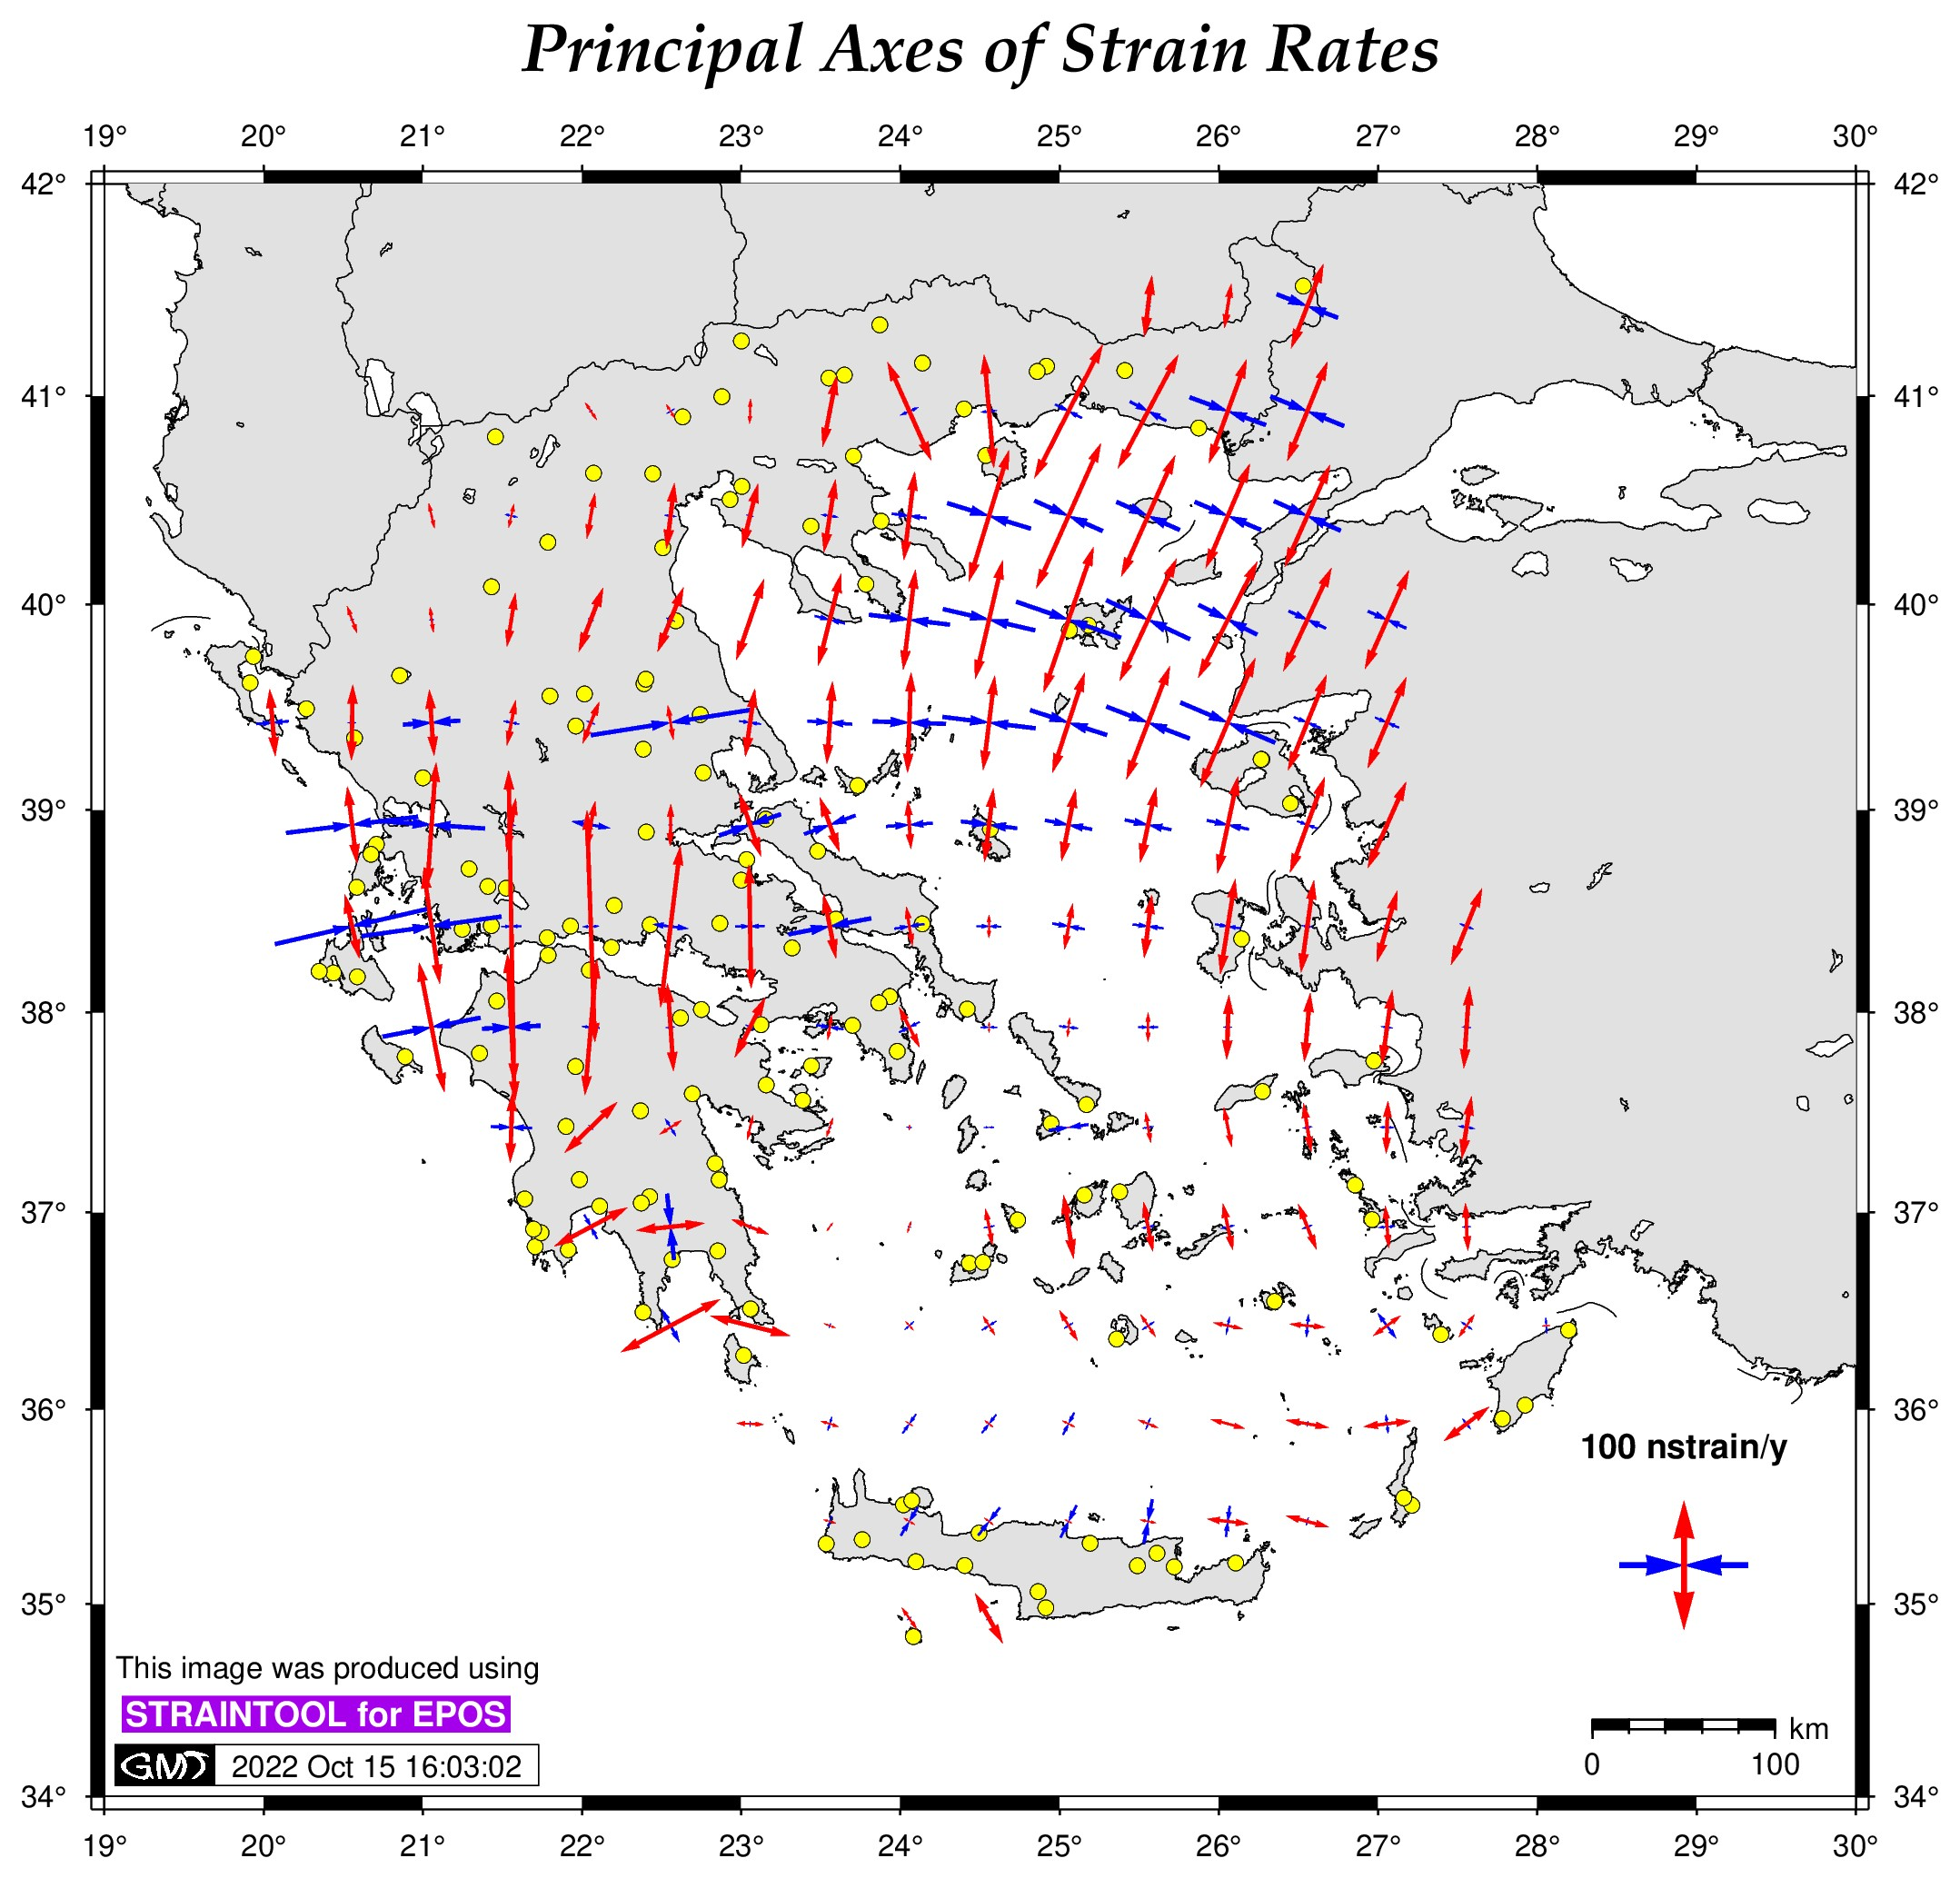
\includegraphics[width=.8\textwidth]{gr-output_str.jpg}
%    \end{center}
%%    \begin{itemize}\setlength\itemsep{1em}
%%      \item \textbf{StrainTool} software used to estimate strain tensor parameters \citep{straintool}
%%      \item grid step 0.5$^{\circ}$
%%    \end{itemize}
%  \end{column}
%  \begin{column}{.5\textwidth}
%    \begin{center}
%      \texttt{DSO\_HPS\_2022}\\
%      
\includegraphics[width=.8\textwidth]{hepos22-output_str.jpg}
%    \end{center}
%  \end{column}
%\end{columns}
%\end{frame}
%\note{}

 % ------------------------------------------------------------------------------
\begin{frame}
  \frametitle{PPP processing for High-rate data}
  \framesubtitle{effect Santorini Volcano crisis (05.02.2025)}
  \label{}\
  \vskip-1cm
  \begin{columns}[T]
    \begin{column}{.49\textwidth}
      \begin{center}
         \texttt{048A\_2025\_035}\\
         
\includegraphics[width=.97\textwidth]{048a_25035.png}
       \end{center} 
    \end{column}
    \begin{column}{.49\textwidth}
      \begin{center}
        \texttt{048A\_2025\_036}\\
        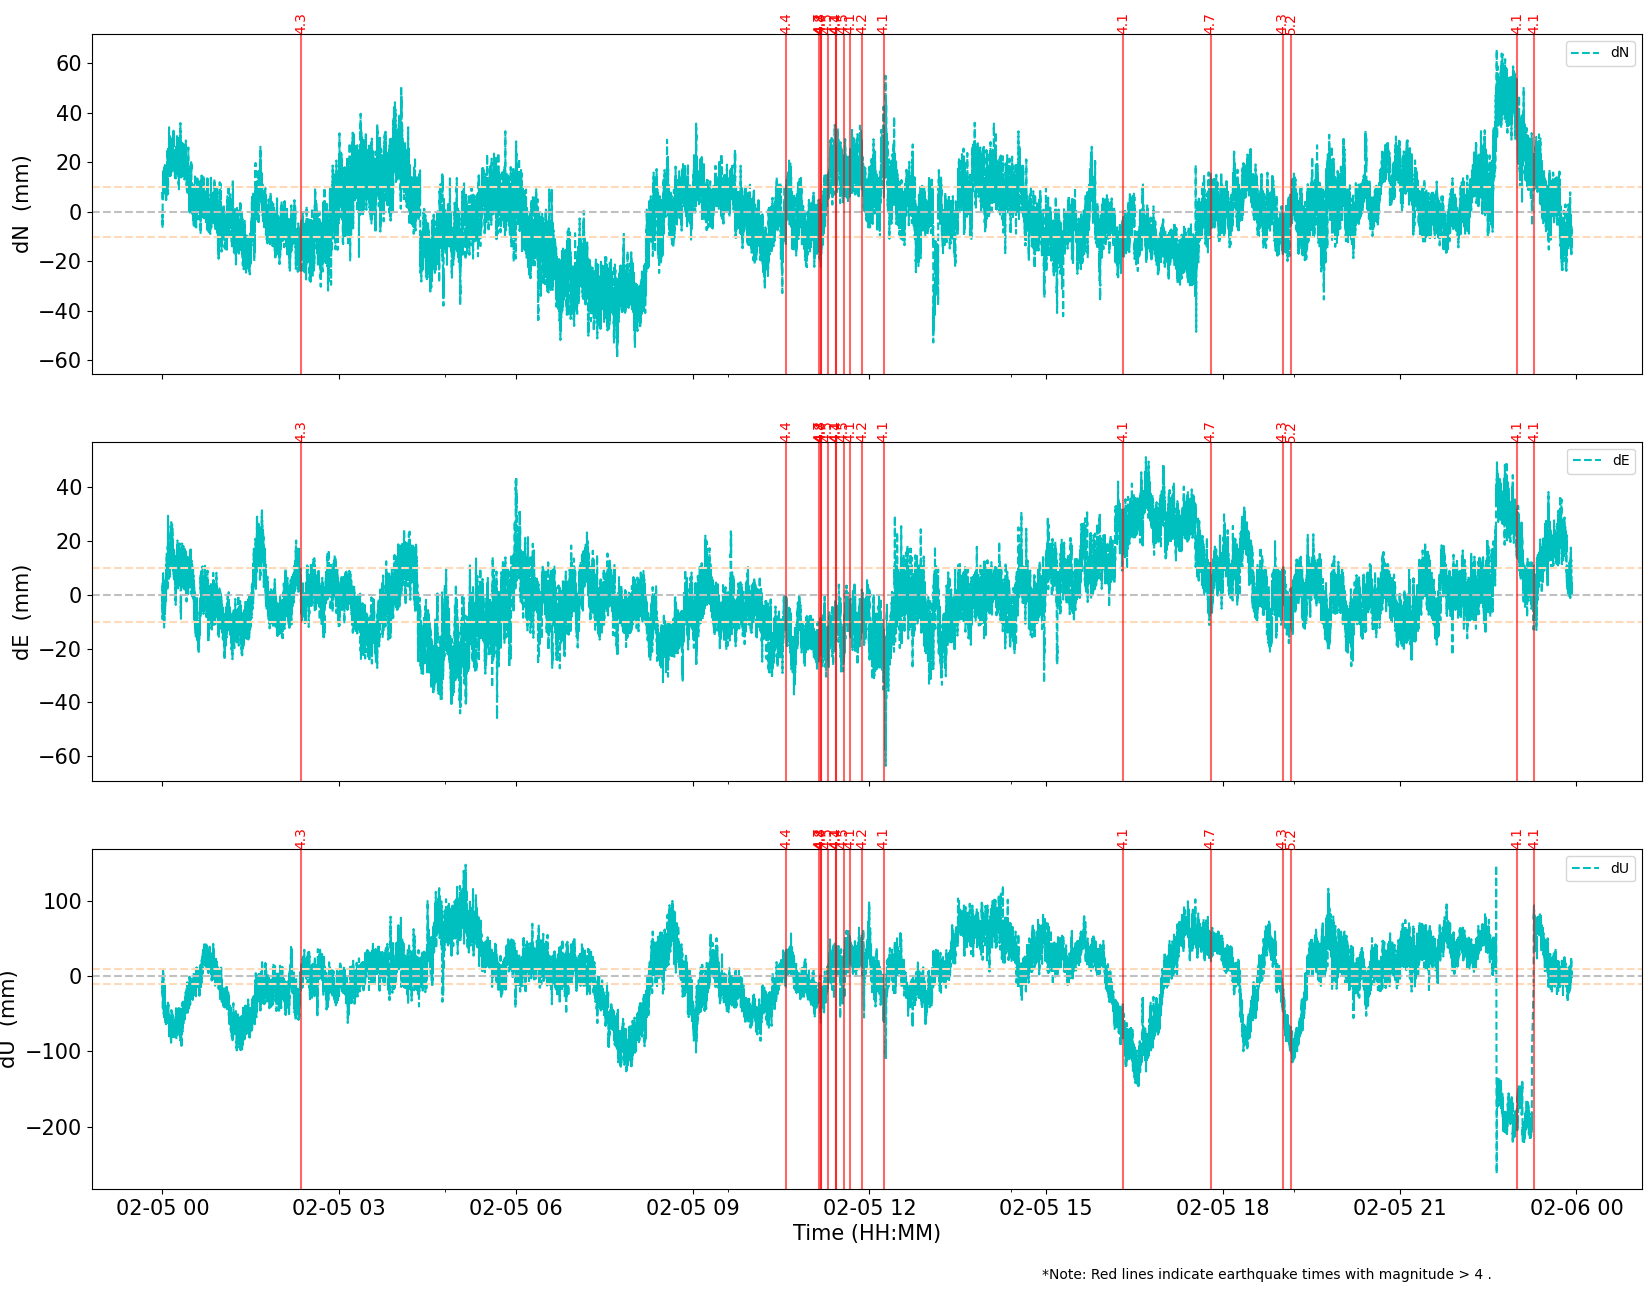
\includegraphics[width=.97\textwidth]{048a_25036.png}
      \end{center}
    \end{column}
  \end{columns}
  \begin{columns}[T]
    \begin{column}{.2\textwidth}
      \begin{center}
        
\includegraphics[width=.97\textwidth]{../../logos/PRIDE.png}
      \end{center}
    \end{column}
    \begin{column}{.8\textwidth}
    \vskip.5cm
      \begin{itemize}\setlength\itemsep{.1em}
        \item 1Hz data available, $\sim$50 stations from HEPOS Netowk.
        \item PPP-AR analysis for 2 days (DOY: 035, 036)
      \end{itemize}
 
    \end{column}
  \end{columns}
\end{frame}
\note{}


 % ------------------------------------------------------------------------------
\begin{frame}
  \frametitle{REPRO2026:Compare velocity field of different networks}
  \framesubtitle{}
  \label{}
  \vskip-1cm
  \begin{columns}[T]
    \begin{column}{.5\textwidth}
    \begin{center}
      \texttt{DSO\_GRC\_2026}\\
      
\includegraphics[width=.97\textwidth]{gr-output_vel.jpg}
    \end{center}
    \end{column}
    \begin{column}{.5\textwidth}
      \begin{center}
        \texttt{DSO\_HPS\_2026}\\
        
\includegraphics[width=.97\textwidth]{hepos22-output_vel.jpg}
      \end{center}    
    \end{column}
  \end{columns}
\end{frame}
\note{}




\section{Discussion / Conclusions}
 % ------------------------------------------------------------------------------
\begin{frame}
  \frametitle{Discussion / Conclusions}
  \framesubtitle{}
  \label{}
  \vskip-.5cm
  \begin{itemize}\setlength\itemsep{.5em}
    \item Greece is located in a complex tectonic background with many changes in the kinematics of the area.
    \item Routine processing and monitoring are very important and revealing for 
      Greece; products are requested by and disseminated to a wide range of Geoscientists.
   %\item Greece's crustal dynamics are evidently complex and inhomogenous; a difficult       task to model by Reference Systems (especially non-dynamic, such as the ones       currently in use).
    \item A dense velocity field for accurate estimation of ground/tectonic motions in the region will help to develop a stable local reference frame and the connection of the region with the global and European reference systems.
    \item The continuous monitoring of the networks gives useful results for the effect of strong earthquakes or other ``abrupt'' phenomena; small, dense networks are of great help (even with instrumentation of non-geodetic accuracy).
    \item DSO is upgrading its scientific output and processing activity via new datasets and real time processing.
      \item  Our plan: grow up our team and be more involved to the GNSS/EUREF community.
  \end{itemize}
\end{frame}
\note{}

